\documentclass[11pt]{article}

\usepackage[margin=1in]{geometry}
\usepackage{hyperref}
\usepackage{booktabs}
\usepackage{longtable}
\usepackage{array}
\usepackage{enumitem}
\usepackage{xcolor}
\usepackage{listings}
\usepackage{parskip}
\usepackage{amsmath}
\usepackage{amssymb}
\usepackage{tikz}
\usetikzlibrary{positioning,arrows.meta,shapes,fit,backgrounds,calc,decorations.pathreplacing}

\tikzset{
  pe/.style={draw,thick,minimum width=1.6cm,minimum height=1.0cm,
            align=center,font=\small,fill=white},
  pebridge/.style={pe,fill=yellow!25,thick,double},
  pecolbridge/.style={pe,fill=cyan!20,thick,double},
  pebackrelay/.style={pe,fill=orange!25},
  peebackrecv/.style={pe,fill=red!10},
  source/.style={->,>=Stealth,thick,blue!70!black},
  bridge/.style={->,>=Stealth,ultra thick,orange!75!black,double},
  backch/.style={->,>=Stealth,thick,red!75!black,dashed},
  colsrc/.style={->,>=Stealth,thick,green!50!black},
  colbridge/.style={->,>=Stealth,ultra thick,teal!75!black,double},
  ramparrow/.style={->,>=Stealth,thick,gray!70},
}

\hypersetup{
  colorlinks=true,
  linkcolor=blue!60!black,
  urlcolor=blue!60!black,
  citecolor=blue!60!black
}

\lstset{
  basicstyle=\ttfamily\small,
  frame=single,
  breaklines=true,
  columns=fullflexible,
  keepspaces=true,
  xleftmargin=0.5em,
  framesep=4pt,
  aboveskip=0.5em,
  belowskip=0.5em
}

\newcommand{\code}[1]{\texttt{#1}}
\newcommand{\file}[1]{\texttt{#1}}

\title{WSE-3 Scaling Analysis: Picasso Graph Coloring on Cerebras}
\author{Picasso / LWW transport working notes}
\date{Last updated: 2026-04-24}

\begin{document}
\maketitle

\begin{abstract}
This document records \textbf{where each of our current kernel
implementations stands against a WSE-3 deployment target}, what
architectural constraints we discovered, how the layout and
algorithm work around them, and what the next concrete steps look
like (bigger test cases, timing plan, on-device recursion
feasibility). It is a working reference: state changes, and every
claim below cites an artifact under \file{runs/local/}.
\end{abstract}

\tableofcontents

\section{A WSE-3 primer (in plain words)}

Before we get into the kernels, let us walk through what WSE-3
actually is and why it forces us to write code the way we do. If
you already know the chip, you can skim. If you do not, every
later section will read more clearly after this.

\subsection{What is WSE-3?}

WSE-3 is one big piece of silicon. It is roughly the size of a
dinner plate. Most chip companies cut a wafer into thousands of
small chips. Cerebras does not. They keep the wafer whole and
treat it as one giant chip. The result is about
\textbf{900{,}000 tiny processors} sitting on one die. We call
each of those processors a \textbf{PE} (short for ``Processing
Element'').

The PEs are arranged in a rectangle of about 750 rows by 990
columns. Each PE is small. It has its own little CPU, around
50~KB of fast on-chip memory, a local scheduler, and four ports
that connect it to its four neighbors (north, south, east, west).
There is no shared memory. There is no central scheduler. PEs
talk to each other only by sending little messages out one port
and receiving them at a neighbor's port.

A useful mental picture is a giant city grid of 900{,}000 small
houses. Each house has four doors, one on each side. Each door
opens onto a short alley that leads to the next-door house.
Every house can talk to every other house, but only by passing
notes hand-to-hand down those alleys.

\begin{center}
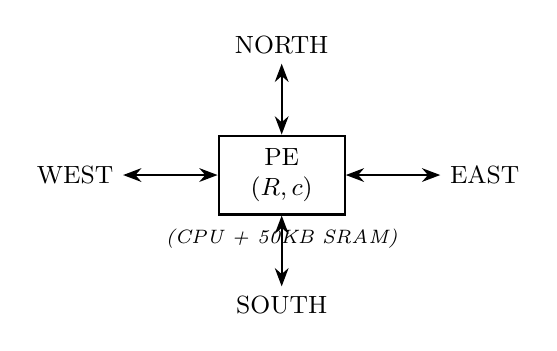
\begin{tikzpicture}[node distance=1.6cm]
  \node[pe] (pe) {PE\\$(R,c)$};
  \node[above=0.9cm of pe,font=\small] (n) {NORTH};
  \node[below=0.9cm of pe,font=\small] (s) {SOUTH};
  \node[left=1.2cm of pe,font=\small] (w) {WEST};
  \node[right=1.2cm of pe,font=\small] (e) {EAST};
  \draw[<->,>=Stealth,thick] (pe.north) -- (n);
  \draw[<->,>=Stealth,thick] (pe.south) -- (s);
  \draw[<->,>=Stealth,thick] (pe.west)  -- (w);
  \draw[<->,>=Stealth,thick] (pe.east)  -- (e);
  \node[font=\scriptsize\itshape,below=0.05cm of pe] {(CPU + 50KB SRAM)};
\end{tikzpicture}
\end{center}

The ``fabric'' is the name we give to all the wires and routers
connecting those PE ports together. When a PE sends a message,
the fabric carries it along to wherever it needs to go.

\subsection{What is a ``wavelet''?}

A \textbf{wavelet} is the unit of message that travels on the
fabric. It is just one 32-bit number. That is all. The PE puts a
32-bit value into one of its output ports, and the fabric
carries that value, hop by hop, to wherever its route says it
should go. Each hop takes a fraction of a nanosecond. By the
time the wavelet arrives at the destination PE, that PE's CPU
can pick it up out of an inbox, look at the bits, and decide
what to do.

Everything that happens on WSE-3 is built out of wavelets going
back and forth. PEs emit wavelets, PEs receive wavelets, PEs do
work in between. There is nothing else on the wires.

\begin{center}
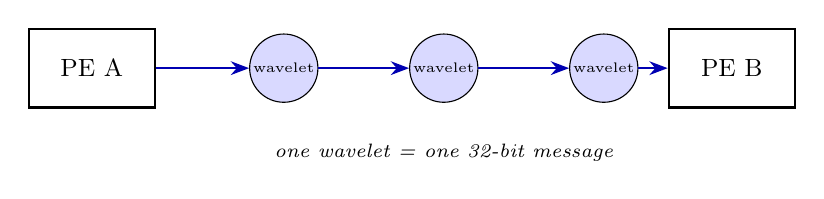
\begin{tikzpicture}[node distance=2.5cm]
  \node[pe] (a) {PE A};
  \node[pe,right=6.5cm of a] (b) {PE B};
  \node[circle,draw,fill=blue!15,inner sep=1pt,font=\tiny]
       (w1) at ($(a)!0.30!(b)$) {wavelet};
  \node[circle,draw,fill=blue!15,inner sep=1pt,font=\tiny]
       (w2) at ($(a)!0.55!(b)$) {wavelet};
  \node[circle,draw,fill=blue!15,inner sep=1pt,font=\tiny]
       (w3) at ($(a)!0.80!(b)$) {wavelet};
  \draw[->,>=Stealth,thick,blue!70!black] (a.east) -- (w1);
  \draw[->,>=Stealth,thick,blue!70!black] (w1) -- (w2);
  \draw[->,>=Stealth,thick,blue!70!black] (w2) -- (w3);
  \draw[->,>=Stealth,thick,blue!70!black] (w3) -- (b.west);
  \node[below=0.4cm of w2,font=\scriptsize\itshape]
       {one wavelet = one 32-bit message};
\end{tikzpicture}
\end{center}

\subsection{Why do we need ``colors''?}

A \textbf{color} is a label stamped on every wavelet. The
fabric's routers look at that label to decide where the wavelet
should go next. You can think of a color like a channel on a
walkie-talkie. If two people are tuned to channel 5, they hear
each other. If one is on channel 5 and one is on channel 7,
they hear nothing from each other.

Why do we need more than one color? Because at any given moment,
a lot of different conversations are happening on the same chip
in parallel. For example, in our graph-coloring kernel:
\begin{itemize}[leftmargin=1.3em,itemsep=0.1em]
  \item Row 3 of PEs might be passing graph-color updates from
    west to east.
  \item Row 4 might be running a global ``are we done?'' check
    from east back to west.
  \item Column 2 might be broadcasting a synchronization bit
    from north to south.
\end{itemize}

All three things have to happen at the same time, on the same
fabric. If they all used the same color, the routers would have
no way to tell them apart. A wavelet might end up going the
wrong direction, or two wavelets might collide on the same wire.
By giving each separate stream its own color, and by setting up
the routers ahead of time to know ``color 5 always goes west,
color 7 always goes east,'' we keep the streams separate.

We use about ten colors in our kernel. WSE-3 gives us only 32
colors total to work with. That is the entire palette for
wiring the chip, so we have to spend them carefully.

\paragraph{The single-source-per-color rule.}
There is one more important rule about colors. It comes from
the way the fabric's routers are configured. \textbf{For any
given color, exactly one PE is allowed to originate new wavelets
on it.} Every other PE that the color's path runs through is
set up either to pass the wavelet along, or to receive the
wavelet at its CPU. No other PE may also start a new wavelet
on the same color.

Why is that? The routers are configured at compile time, before
the program runs. Each router knows ahead of time, for each
color, which direction the wavelets come from and which
direction they go. If two different PEs in two different places
both tried to inject brand new wavelets on the same color, the
routers would get a confused picture of the color's flow. The
wavelets would collide where the two flows met. Some would get
reordered. Some would silently disappear.

In practice this means every color in our kernel has a clear
``owner'' PE. For example, color \code{c\_3\_E} belongs to PE 3,
going east. PE 3 is the only PE allowed to put new wavelets on
\code{c\_3\_E}. PEs further east of PE 3 can only receive on
\code{c\_3\_E}. They cannot also send on it. If PE 4 wants to
send something east, it must use a different color, like
\code{c\_4\_E}.

This single-source rule is the reason a naive one-dimensional
kernel ends up needing $N$ different colors for $N$ PEs in a
row. Each PE needs its own color to be the source. That does
not scale. Later in Section~\ref{sec:east_seg} we will see how
we worked around this by inventing \textbf{bridges} that let us
reuse colors across different parts of the chip.

\paragraph{Single-source rule, in pictures.}

PE 0 sources color $c_0$. PE 1 receives on $c_0$. PE 1 cannot
also be a source for $c_0$.

\begin{center}
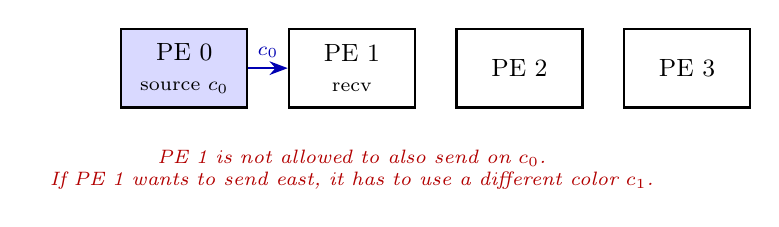
\begin{tikzpicture}[node distance=0.5cm]
  \node[pe,fill=blue!15] (p0) {PE 0\\\scriptsize source $c_0$};
  \node[pe,right=of p0]    (p1) {PE 1\\\scriptsize recv};
  \node[pe,right=of p1]    (p2) {PE 2};
  \node[pe,right=of p2]    (p3) {PE 3};
  \draw[source] (p0) -- node[above,font=\scriptsize] {$c_0$} (p1);
  \node[below=0.4cm of p1,font=\scriptsize\itshape,red!70!black,
        align=center,text width=8cm]
       {PE 1 is not allowed to also send on $c_0$.\\If PE 1 wants
        to send east, it has to use a different color $c_1$.};
\end{tikzpicture}
\end{center}

\vspace{0.4em}

PE 0 sources $c_0$, PE 1 sources $c_1$. Each PE has its own
color.

\begin{center}
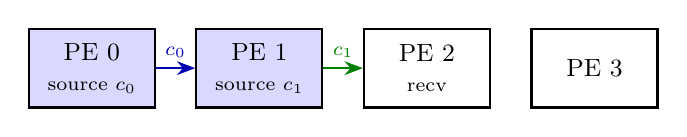
\begin{tikzpicture}[node distance=0.5cm]
  \node[pe,fill=blue!15] (p0) {PE 0\\\scriptsize source $c_0$};
  \node[pe,fill=blue!15,right=of p0] (p1) {PE 1\\\scriptsize source $c_1$};
  \node[pe,right=of p1]    (p2) {PE 2\\\scriptsize recv};
  \node[pe,right=of p2]    (p3) {PE 3};
  \draw[source] (p0) -- node[above,font=\scriptsize] {$c_0$} (p1);
  \draw[source,green!50!black] (p1) -- node[above,font=\scriptsize] {$c_1$} (p2);
\end{tikzpicture}
\end{center}

\subsection{Why do we need queues?}

Wavelets arrive at the CPU very quickly. While a wavelet is
landing, the CPU is usually busy doing something else. Maybe it
is in the middle of speculating a color for one of its local
graph vertices. Maybe it is updating an array in memory. We do
not want to drop the incoming wavelet. We also cannot ask the
fabric to wait. So we need somewhere to park it.

That parking spot is called a \textbf{queue}. It is a small
hardware buffer that holds incoming wavelets until the CPU gets
to them. Each color the PE wants to receive needs its own input
queue (we call them IQs). Each direction the PE wants to send
on needs its own output queue (an OQ).

Queues do another important job. They let the sender and the
receiver work at different speeds. Without a queue, every send
would be like yelling across a room and waiting for the other
person to yell back before you can say anything else. With a
queue, the sender just drops the message in the outbox and goes
on with its work. The receiver picks the message up whenever it
is free. This is what makes the fabric a real pipeline. Many
thousands of wavelets can be in flight at once without anyone
having to wait.

\begin{center}
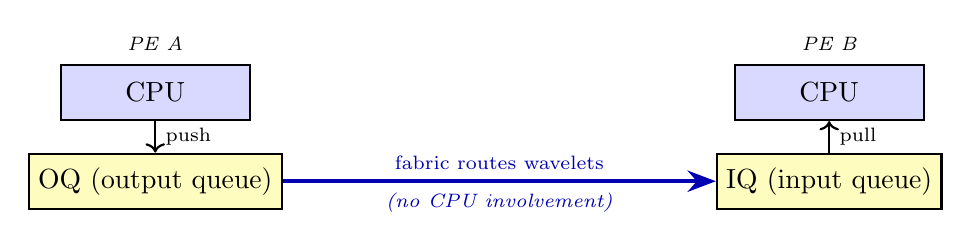
\begin{tikzpicture}[node distance=0.4cm and 0.6cm]
  \node[draw,thick,minimum width=2.4cm,minimum height=0.7cm,
        fill=blue!15] (cpuA) {CPU};
  \node[draw,thick,minimum width=2.4cm,minimum height=0.7cm,
        below=of cpuA,fill=yellow!25] (oq) {OQ (output queue)};
  \node[draw,thick,minimum width=2.4cm,minimum height=0.7cm,
        right=5.5cm of oq,fill=yellow!25] (iq) {IQ (input queue)};
  \node[draw,thick,minimum width=2.4cm,minimum height=0.7cm,
        above=of iq,fill=blue!15] (cpuB) {CPU};
  \draw[->,thick] (cpuA) -- node[right,font=\scriptsize] {push} (oq);
  \draw[->,thick] (iq)   -- node[right,font=\scriptsize] {pull} (cpuB);
  \draw[->,>=Stealth,ultra thick,blue!70!black]
    (oq.east) -- node[above,font=\scriptsize] {fabric routes wavelets}
                node[below,font=\scriptsize\itshape] {(no CPU involvement)} (iq.west);
  \node[above=0.05cm of cpuA,font=\scriptsize\itshape] {PE A};
  \node[above=0.05cm of cpuB,font=\scriptsize\itshape] {PE B};
\end{tikzpicture}
\end{center}

\subsection{Why are queues so limited?}

Every queue is real silicon. It needs a piece of memory to hold
wavelets, a scheduler that decides when to fire the CPU task,
and a slot in the chip's task-ID table. With about 900{,}000
PEs on one die, every byte of per-PE storage adds up to many
megabytes across the whole chip. So Cerebras was very stingy.

\textbf{Each PE gets exactly six input queues and six output
queues that we are allowed to use.} (There are two more of each
that the system reserves for talking to the host computer.)
Six is not a lot.

You can picture it as having only six mailboxes per house in
that 900{,}000-house city. Suppose our program needs to handle
eight different kinds of conversation per PE. For example: row
data going east, column data going south, row reduce going
west, column reduce going north, row broadcast, column
broadcast, the back-channel, and so on. We have eight kinds of
mail but only six mailboxes. Something has to give.

\textbf{Fitting our program into six mailboxes per PE has been
the single biggest engineering challenge of this whole
project.} Almost every implementation step described later in
this document is some new trick for collapsing eight kinds of
mail into six mailboxes.

\subsection{Why are colors also limited?}

Colors are cheaper than queues, but they are still in short
supply. WSE-3 gives us 32 colors total and the system reserves
some, leaving us about 24 we can use. That sounds like a lot
until you remember the single-source rule. If we tried to give
each PE in a row its own color (so that each PE can be the
source of its own east-going stream), then a 990-column row
would need 990 colors. We only have 24. We are off by a factor
of 40.

The way out is \textbf{color reuse}. Two wavelets on the same
color do not collide as long as their paths through the chip
never overlap. So if we can make a color ``live'' only in one
small neighborhood of the chip, and have it ``die'' before it
would collide with the same color used somewhere else, then
the router never sees a conflict.

This is the idea behind the segment-and-bridge design described
later in Section~\ref{sec:east_seg}. We pick a small number,
like four PEs, and let the source colors live only inside
groups of four. At the boundary of each group we have a special
PE called a bridge. The bridge consumes the color, runs
everything it received through its CPU, and starts a fresh
stream on a new color. The next group then reuses the same
source color from scratch. The router never sees two
simultaneous sources on the same color because they are
separated in space by the bridge.

\subsection{How does our algorithm sit on this?}
Picasso's \emph{speculative graph coloring} is a \textbf{BSP loop}
--- Bulk Synchronous Parallel: every PE runs in lock-step rounds
with a global synchronization barrier between rounds. Each round
is

\begin{quote}
\emph{guess a color, tell neighbors, detect conflicts, revert
losers, repeat until stable.}
\end{quote}

Each round is a wavelet exchange followed by a \textbf{reduce}
then a \textbf{broadcast} (terms defined below).

\paragraph{Reduce.} ``Reduce'' is the parallel-computing word for
\emph{combining many values into one}. Example: every PE has a
flag ``do I still have an uncolored vertex? (yes/no).'' The reduce
step asks the global question \emph{``is anyone still
uncolored?''} by OR'ing every PE's flag into a single bit. The OR
is the ``reduction operator'', sum and max are other common
reductions. On a fabric, a reduce is implemented as a chain of
wavelets: each PE receives the partial OR from its neighbor, OR's
in its own bit, and forwards the result onward.

\paragraph{Broadcast.} Once one PE knows the global answer
(``yes, run another round''), it has to \textbf{tell every other
PE}. That is a broadcast, the same value sent to many
recipients. On a fabric it is the reverse direction of the reduce:
one wavelet starts at one PE and propagates outward.

\paragraph{Mapped onto WSE-3:}
\begin{itemize}[leftmargin=1.3em,itemsep=0.15em]
  \item \textbf{Guess:} PE runs locally, no fabric traffic.
  \item \textbf{Tell neighbors:} one wavelet per boundary edge on
    a color that routes toward that neighbor.
  \item \textbf{Detect + revert:} PE runs locally again.
  \item \textbf{Reduce + broadcast:} a short chain of wavelets
    along the row (and column, in 2D), accumulating at each PE for
    the reduce, then a second chain in the reverse direction for
    the broadcast.
\end{itemize}

The kernel's job is to make the ``tell neighbors'' + ``reduce +
broadcast'' traffic fit in the 6-queue / $\sim\!10$-color budget
at any grid size we pick. \textbf{That is the engineering problem
the rest of this document spells out.}

\subsection{Glossary}

Quick definitions for the recurring jargon, every time one of
these words appears later in the document, it means what it says
here.

\begin{longtable}{p{4.0cm} p{10.5cm}}
\toprule
Term & Plain meaning \\
\midrule
\endhead
\textbf{PE} & ``Processing Element'', one of the $\sim\!900{,}000$ small CPUs on a WSE-3 die. \\
\textbf{Wavelet} & A 32-bit message sent from one PE to a neighbor over the fabric. The unit of fabric traffic. \\
\textbf{Fabric} & The on-die mesh of routers (one per PE) that delivers wavelets between PEs. \\
\textbf{Color} & A label stamped on a wavelet that tells the routers how to route it. Like a walkie-talkie channel. \\
\textbf{Queue (IQ / OQ)} & Small hardware buffer that holds incoming (IQ) or outgoing (OQ) wavelets while the CPU is busy. WSE-3 has 6 user IQs and 6 user OQs per PE. \\
\textbf{Route} & The per-PE configuration that says ``for color $X$, accept wavelets from direction $Y$ and send them out direction(s) $Z$.'' Configured by the layout file at compile time. \\
\textbf{RAMP} & A special ``direction'' name for the PE's own CPU. \code{rx=RAMP} means the CPU originates wavelets on this color; \code{tx=RAMP} means deliver these wavelets to the CPU. \\
\textbf{BSP} & Bulk Synchronous Parallel, every PE runs a round of work, syncs at a barrier, runs the next round, etc. \\
\textbf{Round} & One pass of the BSP loop. Within a level, Picasso may take several rounds to resolve all conflicts. \\
\textbf{Level} & One Picasso recursion stage. Each level uses a smaller palette and processes the vertices that remain uncolored after previous levels. \\
\textbf{Reduce} & A collective that combines a value from every PE into one global value (e.g.\ OR of all ``uncolored?'' flags). Implemented as a wavelet chain. \\
\textbf{Broadcast (bcast)} & A collective that distributes one PE's value to all PEs. Reverse direction of a reduce. \\
\textbf{Boundary} & A vertex on PE $A$ whose graph neighbor lives on PE $B$. Boundaries are the only vertices whose color updates need to leave the PE. \\
\textbf{Speculative coloring} & The PE picks a color guess locally, sends to neighbors, and finds out later whether it conflicts. The ``loser'' reverts and re-guesses next round. \\
\textbf{Path C} & Our partitioning rule: assign vertices to PEs by contiguous GID ranges in row-major order so that ``lower-GID wins'' automatically becomes ``western (or northern) PE wins.'' \\
\textbf{GID} & Global vertex ID. A unique integer assigned to every graph vertex. \\
\textbf{Segment} & A run of $S$ consecutive PEs along an axis that share a small set of source colors. Segments let us reuse colors instead of allocating one per PE. \\
\textbf{Bridge} & The last PE of a segment. Receives wavelets on the in-segment colors, re-emits them on a \emph{bridge color} so the next segment can decode the merged stream. \\
\textbf{Bridge color reuse} & Bridge color $c_{be}$ is alive only between bridge $k$ and bridge $k{+}1$. Bridge $k{+}2$ can reuse $c_{be}$ because the previous use has terminated. \\
\textbf{Back-channel} & A wavelet path that flows \emph{opposite} to the main data direction (here, westward through a row whose data flows east). Needed for ``south-west'' anti-diagonal cross-PE conflicts where the winner sits east of the loser. \\
\textbf{e2s relay} & ``East to South'' relay. A PE that re-emits east-arriving wavelets onto the south-going stream so columns east of the sender also receive them. \\
\textbf{In-band opcode} & A scheme where a few bits of the 32-bit wavelet are reserved as a ``type tag'' so multiple logical streams (data, data-done, broadcast, reduce) can share one fabric color. The CPU dispatches on the bit pattern. \\
\textbf{LWW} & ``Last Writer Wins'', the conflict-resolution rule. When two PEs claim the same color for adjacent boundary vertices, the higher-GID PE reverts. Today this is just ``lower-GID wins'' plus speculative guessing. \\
\textbf{Pipelined-LWW} & Our family of fabric-pipelined kernels (as opposed to \code{sw-relay} which involves the host between every hop). \\
\textbf{Data-done sentinel} & A special wavelet (one per PE per round) that says ``I have finished sending all my data wavelets for this round.'' Receivers count these to know when it is safe to detect conflicts. \\
\textbf{Round-parity tag} & One bit (\code{[30]=parity}) on every wavelet that says ``round even'' or ``round odd.'' Lets a fast PE send round-$k{+}1$ wavelets before a slow PE finishes round-$k$ without confusing the receiver. \\
\textbf{OQ backpressure} & When the OQ is full, the CPU's next \code{@mov32} send call blocks until the fabric drains. Not a bug, but a perf cliff under heavy traffic. \\
\bottomrule
\end{longtable}

\section{Summary: which implementations scale to WSE-3?}

We maintain three parallel kernel families under
\file{picasso/run\_csl\_tests.py}.

\begin{longtable}{p{3.4cm} p{5.2cm} p{2.3cm} p{3.8cm}}
\toprule
Routing / layout & Files & Dim support & Scales to WSE-3? \\
\midrule
\endhead
\code{sw-relay} (baseline) & \file{csl/layout.csl}, \file{csl/pe\_program.csl} & 1D and 2D any $N$ & \textbf{Yes (trivially)}, every PE is independent, no color/queue pressure. Slow but correct. \\
\code{hw-filter} & \file{csl/layout\_hw\_broadcast.csl} et al. & 1D only & No, 2D would need multicast switches we do not use. Out of scope. \\
\code{pipelined-lww} & family below & varies & \textbf{Yes, at $S=2$ dual-axis} (\code{2d\_seg2}). \\
\bottomrule
\end{longtable}

\subsection{Pipelined-LWW sub-variants}

\begin{longtable}{p{2.4cm} p{3.7cm} p{2.2cm} p{1.6cm} p{4.0cm}}
\toprule
\code{--lww-layout} & Dim support & Validated at & Scales & Notes \\
\midrule
\endhead
\code{bidir} & 1D, $\le 5$ PEs & $1\times 4$ & No & Bidirectional east+west; killed by 6-queue cap beyond 5 PEs + CP3 reinject rule. \\
\code{east} & 1D, $\le 5$ PEs & $1\times 4$ & No & Single-segment east-only. \\
\code{east\_seg} & 1D, any width & $1\times 16$ & \textbf{Yes} & Segmented east-only with bridge-color alternation. Queue use constant per PE. \\
\code{2d} & $2\times 2$ only & $2\times 2$ & No & Iter-2 fixed plumbing. \\
\code{2d\_seg} & single-axis & $1\times 16$, $16\times 1$ & \textbf{Yes} & Axis-agnostic segmented east/south. \\
\code{2d\_seg2} & dual-axis $2\times 2\ldots 16\times 16$ & through $16\times 16$ sparse & \textbf{Yes} & $S=2$ segments, merged back-channel on reduce chain, in-band row/col bcast. \\
\code{2d\_multicast} & 2D small grids & $4\times 4$ probe & Partial & Multicast switches; 4-way fanout capped at $5\times 5$. Not the chosen path. \\
\bottomrule
\end{longtable}

\textbf{Short answer.} For WSE-3, \code{--lww-layout 2d\_seg2} is
the design that actually closes the queue, color, and route budget
at $S=2$ with a \emph{grid-size-invariant} kernel. The same
compiled binary runs at $2\times 2$, $4\times 4$, $8\times 8$,
$16\times 16$, and $2\times 16$ today; larger sizes are simulator-
bound but architecturally identical.

\section{The implementation story, how we got here, step by step}

This section walks through every kernel we have built, in the
order we built them. Each one was written \textbf{to solve a
specific limitation of the one before it}. By the end you should
see exactly \emph{why} the design ended up the way it did.
none of the choices were arbitrary; each one came from running
into a wall with the previous design and looking for the smallest
change that would let us climb over it.

The walls we kept hitting are always one (or two) of:

\begin{enumerate}[leftmargin=1.3em,itemsep=0.15em]
  \item \textbf{Six queues per PE.} Every distinct color we want
    the CPU to receive on, or send on, costs one queue. If we end
    up wanting eight kinds of conversation per PE, two of them
    have to share somehow.
  \item \textbf{One source per color.} A color belongs to exactly
    one PE in any given route. We cannot just ``add another
    sender'', we have to invent a new color, or have the CPU
    re-emit on a different color (a \emph{bridge}).
  \item \textbf{One rx-direction per color.} For a single color
    at a single PE, the route accepts wavelets from at most one
    side (\code{EAST}, \code{WEST}, \code{NORTH}, \code{SOUTH},
    or \code{RAMP}). This is what forces \emph{alternating}
    color chains for any operation where the CPU has to receive
    \emph{and} re-send on the same logical stream.
  \item \textbf{Total color budget $\sim\!24$.} Once we run out
    of colors, the only way forward is to reuse them on
    disjoint regions of the grid.
\end{enumerate}

Keep these four walls in mind as you read, every jump from one
implementation to the next was a way around one of them.

\subsection{\code{sw-relay}, start with something that just works}
\textbf{Files:} \file{csl/layout.csl}, \file{csl/pe\_program.csl}.

The first thing we needed was a kernel that produced
\emph{correct} colorings at any grid size. Speed could come
later. So \code{sw-relay} does the simplest thing that works:
each PE owns its local vertices, and when a vertex on PE $A$
needs to know about a boundary neighbor on PE $B$, the wavelet
travels one hop on the fabric, and the host (or a small CPU
task) reads it and decides what to do next. The ``SW'' in
\code{sw-relay} means \textbf{software relay}: multi-hop traffic
is not pipelined on the fabric, every hop involves a software
step.

For colors and queues this kernel is generous. It uses an
eight-color checkerboard for east/west/north/south data
(alternating even/odd colors by PE parity so adjacent PEs do not
try to send and receive on the same color at the same moment).
Three more colors handle the global synchronization barrier.
Per-PE we use about four data queues plus one or two for the
barrier. We are nowhere near the 6-queue cap.

The reason \code{sw-relay} is still in the repo is that it works
at \emph{any} grid size and \emph{any} aspect ratio, so it
remains our correctness oracle: when a new pipelined kernel
produces a suspicious coloring, we run the same graph through
\code{sw-relay} and diff. The reason it is \textbf{not} the
scaling target is exactly that ``every hop involves software.''
On big fabrics with many hops, the software step becomes the
bottleneck. We want the wavelets to fly across the fabric without
CPUs in the loop. That want is what motivates everything else.

\paragraph{Layout sketch (1D, 4 PEs).}
Eight data colors form a checkerboard. Adjacent PEs use opposite-
parity colors so a sender and a receiver are never trying to use
the same color in the same instant. Three more colors carry the
global synchronization barrier (not drawn).

\begin{center}
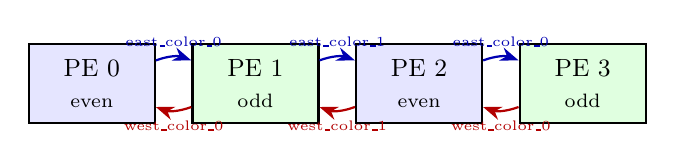
\begin{tikzpicture}[node distance=0.45cm,every node/.style={font=\footnotesize}]
  \node[pe,fill=blue!10] (p0) {PE 0\\\scriptsize even};
  \node[pe,fill=green!12,right=of p0] (p1) {PE 1\\\scriptsize odd};
  \node[pe,fill=blue!10,right=of p1]  (p2) {PE 2\\\scriptsize even};
  \node[pe,fill=green!12,right=of p2] (p3) {PE 3\\\scriptsize odd};
  \draw[source] (p0) to[bend left=20]
        node[above,font=\tiny]{east\_color\_0} (p1);
  \draw[source] (p1) to[bend left=20]
        node[above,font=\tiny]{east\_color\_1} (p2);
  \draw[source] (p2) to[bend left=20]
        node[above,font=\tiny]{east\_color\_0} (p3);
  \draw[->,>=Stealth,thick,red!70!black] (p1) to[bend left=20]
        node[below,font=\tiny]{west\_color\_0} (p0);
  \draw[->,>=Stealth,thick,red!70!black] (p2) to[bend left=20]
        node[below,font=\tiny]{west\_color\_1} (p1);
  \draw[->,>=Stealth,thick,red!70!black] (p3) to[bend left=20]
        node[below,font=\tiny]{west\_color\_0} (p2);
\end{tikzpicture}
\end{center}

\paragraph{Per-PE queue use (any interior PE).}
\begin{center}\footnotesize
\begin{tabular}{ll}
\toprule
Queue & Purpose \\
\midrule
2 IQ (east + west data) & receive from both neighbors \\
2 OQ (east + west data) & send to both neighbors \\
1 IQ (barrier reduce)   & global sync, in-bound \\
1 OQ (barrier broadcast) & global sync, out-bound \\
\midrule
total & 6 queues, well inside the 6-queue cap \\
\bottomrule
\end{tabular}
\end{center}

The CPU does software relay: when it receives a wavelet, it
inspects the sender ID and decides whether to forward the
wavelet to the next hop. The host is in the loop on every hop,
which is why \code{sw-relay} is correct but slow.

\subsection{\code{pipelined-lww bidir}, the first attempt at a fabric pipeline}
\textbf{Files:} \file{csl/layout\_lww.csl},
\file{csl/pe\_program\_lww.csl}.

So we asked: can each PE just \emph{broadcast} its colored
vertices into the fabric, in both directions, and let the
receiving PEs filter for the wavelets they care about? That is
what \code{bidir} is. Every PE $k$ owns \textbf{its own
east-going color} \code{c\_k\_E} and \textbf{its own west-going
color} \code{c\_k\_W}. PE $k$ injects every newly colored
boundary vertex onto both colors. PE $k{+}1$ receives PE $k$'s
east color from its west door, scans its boundary list, and
keeps only the wavelets whose sender ID matches a graph neighbor
it cares about. PE $k{-}1$ does the same with PE $k$'s west
color.

This is the first place we ran into the
\textbf{single-source-per-color rule} in practice. We could not
just say ``everyone sends on \code{c\_E}'' and let the fabric
figure it out, the routes have to be preconfigured to know
exactly which PE originates each color, so there must be one
color per source PE. That immediately means \textbf{each PE
consumes one color slot per direction} ($2N$ colors total for an
$N$-PE row), and \textbf{each interior PE needs one input queue
per remote sender it might hear from} ($N{-}1$ for east-plus-west
neighbors combined, in the worst case).

For 4 PEs in a row that is 8 data colors plus 3 barrier.
fine. For 5 PEs it is 10 + 3 = 13, still under the $\sim\!24$
usable colors but starting to pinch. For 6 PEs an interior PE
needs 5 input queues just for data plus 2 for the barrier.
already 7, \emph{one over} the 6-queue cap.

So \code{bidir} worked beautifully up to 4--5 PEs in a row and
proved that the fabric pipeline is genuinely faster than
\code{sw-relay} ($1.1\times$--$1.4\times$ speedup on tests
1--10, recorded in Section~\ref{sec:timing-1d}). It also
introduced a piece of machinery we kept ever after: the
\textbf{round-parity tag}, one bit on every wavelet that says ``I
belong to round $k$ even'' or ``I belong to round $k$ odd.''
Without it, a fast PE that finished round $k$ early might emit
round-$k{+}1$ wavelets while its slow neighbor was still
processing round $k$; the receiver would mis-attribute the early
wavelet and lose a flag. With the parity bit, the receiver can
park ``wrong-parity'' wavelets in a staging buffer until its
\code{reset\_round\_state} runs.

But \code{bidir} could not scale past five PEs, and we wanted to
color graphs much bigger than that. So we asked the next
question.

\paragraph{Layout sketch (1D, 4 PEs).}
Each PE owns its own east-going color and its own west-going
color. Every PE broadcasts on both. Downstream receivers filter
by sender ID at the CPU.

\begin{center}
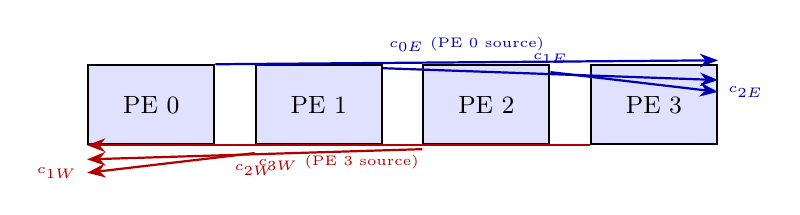
\begin{tikzpicture}[node distance=0.5cm,every node/.style={font=\footnotesize}]
  \node[pe,fill=blue!12] (p0) {PE 0};
  \node[pe,fill=blue!12,right=of p0] (p1) {PE 1};
  \node[pe,fill=blue!12,right=of p1] (p2) {PE 2};
  \node[pe,fill=blue!12,right=of p2] (p3) {PE 3};
  % East colors per source (drawn as long arrows extending past their immediate neighbor)
  \draw[source] (p0.north east) -- ($(p3.north east)+(0,0.05)$)
    node[midway,above,font=\tiny]{$c_{0E}$ (PE 0 source)};
  \draw[source] (p1.north east)+(0,-0.05) -- ($(p3.north east)+(0,-0.20)$)
    node[midway,above,font=\tiny]{$c_{1E}$};
  \draw[source] (p2.north east)+(0,-0.10) -- ($(p3.north east)+(0,-0.35)$)
    node[right,font=\tiny]{$c_{2E}$};
  % West colors per source
  \draw[->,>=Stealth,thick,red!70!black]
    (p3.south west) -- ($(p0.south west)+(0,0)$)
    node[midway,below,font=\tiny]{$c_{3W}$ (PE 3 source)};
  \draw[->,>=Stealth,thick,red!70!black]
    (p2.south west)+(0,-0.05) -- ($(p0.south west)+(0,-0.18)$)
    node[midway,below,font=\tiny]{$c_{2W}$};
  \draw[->,>=Stealth,thick,red!70!black]
    (p1.south west)+(0,-0.10) -- ($(p0.south west)+(0,-0.35)$)
    node[left,font=\tiny]{$c_{1W}$};
\end{tikzpicture}
\end{center}

\paragraph{Per-PE queue use (interior PE 1 of 4).}
\begin{center}\footnotesize
\begin{tabular}{ll}
\toprule
Queue & Bound to \\
\midrule
1 OQ & own east-going color $c_{1E}$ \\
1 OQ & own west-going color $c_{1W}$ \\
1 IQ & receive from PE 0 east color $c_{0E}$ \\
1 IQ & receive from PE 2 west color $c_{2W}$ \\
1 IQ & receive from PE 3 west color $c_{3W}$ \\
1 IQ + 1 OQ & barrier reduce / broadcast \\
\midrule
total & 4 IQs + 3 OQs \\
\bottomrule
\end{tabular}
\end{center}

For 5 PEs in a row this just fits. For 6 PEs it no longer fits:
the interior PE would need 5 east+west IQs, and we are out of
queue slots.

\subsection{\code{pipelined-lww east}, half the colors by exploiting Path C}
\textbf{Files:} \file{csl/layout\_lww\_east.csl},
\file{csl/pe\_program\_lww\_east.csl}.

Why are we sending wavelets \emph{both} directions when the
conflict rule already says ``higher-GID always loses''? If we
assign vertex IDs in row-major order (PE 0 owns the lowest IDs,
PE 1 the next chunk, ..., PE $N{-}1$ the highest), then for any
cross-PE conflict, the eastern PE has the higher ID and will be
the one to revert. The eastern PE \emph{needs} to hear from the
western PE in order to detect the conflict. The western PE does
\textbf{not} need to hear from the eastern PE, it cannot
lose, so it has nothing to do with the news.

We named this the \textbf{Path C invariant}.
\emph{contiguous monotone GID allocation guarantees the western
PE always wins.} Once we adopted Path C in the host partitioner,
the entire westbound half of \code{bidir} became dead weight.
Dropping it gave us \code{pipelined-lww east}: same per-PE color
scheme as \code{bidir}, but only the east-going half. The color
count drops from $2N$ to $N$; the queue count drops by half on
the data side.

Does this scale further? Not really. With $N{-}1$ remote
east-senders to listen to, an interior PE still needs $N{-}1$
input queues just for east data, and the barrier still needs two
more. At 6 PEs you are already at 7 IQs. The cap shifted from
``5 PEs'' to ``5 PEs with a little more headroom''.
fundamentally the same wall.

But what \code{east} taught us was very valuable: \textbf{the
partitioning choice on the host can collapse half the fabric
traffic on the device.} That was the door to color-reuse. If we
are no longer trying to hear from every other PE individually,
maybe we do not need a separate color per sender at all.

\paragraph{Layout sketch (1D, 4 PEs).}
Same as \code{bidir} but with the entire westbound half deleted.
Each PE owns one east-going color. Path C on the host guarantees
the eastern PE in any conflict is the loser, so westbound data
is provably redundant.

\begin{center}
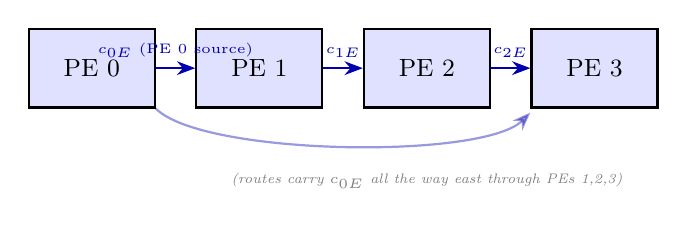
\begin{tikzpicture}[node distance=0.5cm,every node/.style={font=\footnotesize}]
  \node[pe,fill=blue!12] (p0) {PE 0};
  \node[pe,fill=blue!12,right=of p0] (p1) {PE 1};
  \node[pe,fill=blue!12,right=of p1] (p2) {PE 2};
  \node[pe,fill=blue!12,right=of p2] (p3) {PE 3};
  \draw[source] (p0.east) -- node[above,font=\tiny]{$c_{0E}$ (PE 0 source)} (p1.west);
  \draw[source] (p1.east) -- node[above,font=\tiny]{$c_{1E}$} (p2.west);
  \draw[source] (p2.east) -- node[above,font=\tiny]{$c_{2E}$} (p3.west);
  % And the long-haul arrows showing PE 0's color reaches PE 3 too
  \draw[source,opacity=0.4] (p0.south east) ..controls +(0.6,-0.6) and +(-0.6,-0.6)..
        ($(p3.south west)+(0,-0.05)$);
  \node[below=0.7cm of p2,font=\tiny\itshape,gray]
        {(routes carry $c_{0E}$ all the way east through PEs 1,2,3)};
\end{tikzpicture}
\end{center}

\paragraph{Per-PE queue use (interior PE 1 of 4).}
\begin{center}\footnotesize
\begin{tabular}{ll}
\toprule
Queue & Bound to \\
\midrule
1 OQ & own east-going color $c_{1E}$ \\
1 IQ & receive from PE 0 east color $c_{0E}$ \\
1 IQ + 1 OQ & barrier reduce / broadcast \\
\midrule
total & 2 IQs + 2 OQs \\
\bottomrule
\end{tabular}
\end{center}

Half the queues of \code{bidir}, but per-PE queues still grow
linearly with $N$. At 6 PEs an interior PE needs 5 east IQs,
which puts us back over the queue cap.

\subsection{\code{pipelined-lww east\_seg}. Break the per-PE color tax with bridges}
\label{sec:east_seg}
\textbf{Files:} \file{csl/layout\_lww\_east\_seg.csl},
\file{csl/pe\_program\_lww\_east\_seg.csl}.

This is the design that finally scales 1D to any number of PEs.
It is built on one big idea: \textbf{reuse colors across the
chip by letting them die at well-chosen points and starting
fresh ones}.

Here is how it works. We pick a small number called the
\textbf{segment size}, written $S$. In our 1D kernel we use
$S = 4$. In the 2D kernel we use $S = 2$. Then we chop the row
of PEs into segments, each of which contains $S$ PEs in a row.

Inside one segment, the PE at the first position injects new
wavelets on color $c_0$. The PE at the second position injects
on $c_1$. The third uses $c_2$. The fourth uses $c_3$. The
downstream PEs in the same segment receive on those colors. So
far this is just like the \code{east} kernel, except that we
only need $S$ colors instead of $N$.

The trick is the \textbf{bridge}. The last PE of every
non-final segment is treated specially. It does not inject
anything new on its own source color toward the next segment.
Instead, its CPU listens on every color that flowed into the
segment, and for each wavelet it receives it re-emits a copy on
a new color called the \textbf{bridge color}. The bridge color
is shared across the rest of the chip according to a clever
alternation: the first bridge uses \code{c\_be}, the second
uses \code{c\_bo}, the third uses \code{c\_be} again, the
fourth uses \code{c\_bo} again, and so on. We alternate between
just two bridge colors no matter how many segments there are.

Once the bridge has consumed everything from segment 0 and
re-emitted on \code{c\_be}, the source colors $c_0, c_1, c_2,
c_3$ are no longer ``alive'' anywhere east of the bridge. So
the next segment is free to reuse those same source colors
from scratch. The router never sees a collision because the
two uses of $c_0$ are separated by the bridge.

The bridge colors do the same trick one level up.
\code{c\_be} is alive only between bridge $k$ and bridge
$k{+}1$. At bridge $k{+}1$ the CPU consumes \code{c\_be} and
starts a new flow on \code{c\_bo}. So bridge $k{+}2$ can reuse
\code{c\_be} again without conflict. Two bridge colors
alternating in this pattern is enough for any number of
segments.

A picture might help. Here is a row of 8 PEs split into two
segments of 4 with one bridge between them:

\begin{center}
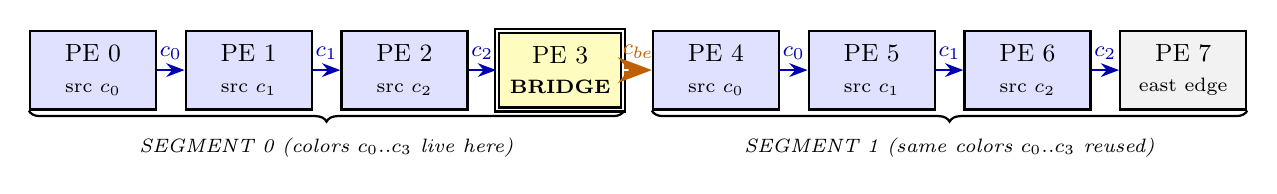
\begin{tikzpicture}[node distance=0.35cm,every node/.style={font=\footnotesize}]
  % Segment 0 PEs
  \node[pe,fill=blue!12]              (p0) {PE 0\\\scriptsize src $c_0$};
  \node[pe,fill=blue!12,right=of p0]   (p1) {PE 1\\\scriptsize src $c_1$};
  \node[pe,fill=blue!12,right=of p1]   (p2) {PE 2\\\scriptsize src $c_2$};
  \node[pebridge,right=of p2]          (p3) {PE 3\\\scriptsize \textbf{BRIDGE}};
  % Segment 1 PEs
  \node[pe,fill=blue!12,right=of p3]   (p4) {PE 4\\\scriptsize src $c_0$};
  \node[pe,fill=blue!12,right=of p4]   (p5) {PE 5\\\scriptsize src $c_1$};
  \node[pe,fill=blue!12,right=of p5]   (p6) {PE 6\\\scriptsize src $c_2$};
  \node[pe,fill=gray!10,right=of p6]   (p7) {PE 7\\\scriptsize east edge};
  % Source-color arrows inside segment 0
  \draw[source] (p0) -- node[above]{$c_0$} (p1);
  \draw[source] (p1) -- node[above]{$c_1$} (p2);
  \draw[source] (p2) -- node[above]{$c_2$} (p3);
  % Bridge re-emit
  \draw[bridge] (p3) -- node[above]{$c_{be}$} (p4);
  % Source-color arrows inside segment 1 (REUSED colors)
  \draw[source] (p4) -- node[above]{$c_0$} (p5);
  \draw[source] (p5) -- node[above]{$c_1$} (p6);
  \draw[source] (p6) -- node[above]{$c_2$} (p7);
  % Segment brackets
  \draw[decorate,decoration={brace,amplitude=4pt,mirror},thick]
    (p0.south west) -- (p3.south east)
    node[midway,below=6pt,font=\scriptsize\itshape] {SEGMENT 0 (colors $c_0..c_3$ live here)};
  \draw[decorate,decoration={brace,amplitude=4pt,mirror},thick]
    (p4.south west) -- (p7.south east)
    node[midway,below=6pt,font=\scriptsize\itshape] {SEGMENT 1 (same colors $c_0..c_3$ reused)};
\end{tikzpicture}
\end{center}

\textbf{Reading the diagram.} Source colors $c_0$, $c_1$, $c_2$
fan out from each PE to its right-hand neighbor inside one
segment. They die at the bridge (PE~3), which reads every
incoming wavelet on its CPU and re-emits it on the bridge
color $c_{be}$. From PE~4 onward the same source colors
$c_0$, $c_1$, $c_2$ start fresh because the previous uses are
gone. The router never sees two simultaneous sources of $c_0$
because the bridge acts as a clean cut between segments.

The numbers come out cleanly. We use $S$ source colors plus
two bridge colors plus three barrier colors. That is
\textbf{nine colors total no matter how wide the row is}.
The per-PE queue count is also constant. An interior bridge
PE needs two output queues (one for east data, one for the
reduce chain). It also needs six input queues (the reduce
receiver, the broadcast receiver, and four data-slot
receivers that cover the bridge color plus the in-segment
source colors). That fills exactly six out of six input queues
at $S = 4$. We cannot grow $S$ any further in this kernel
without breaking the queue cap, but we can grow $N$ as much
as we want by adding more segments. The total chip width
becomes unbounded.

This was the first kernel that ran a $1 \times 16$ row from
end to end. It also locked in the \textbf{segment plus
bridge} pattern that every later 2D kernel inherits. We did
pay one cost. The bridge PE has to do CPU work for every
wavelet that crosses it. The CPU receives the wavelet on one
color, writes it briefly to memory, and emits it on a
different color. That is slower than a pure fabric forward
where the wavelet would just sail through the routers without
any CPU involvement. But CPU re-emission is the price we pay
to dodge the single-source rule with a finite color budget.

\paragraph{Per-PE queue use.}
Per-PE queue counts now stay constant regardless of $N$.

\begin{center}\footnotesize
\begin{tabular}{lll}
\toprule
PE position & Queues used & Notes \\
\midrule
in-segment (non-bridge) & 2 IQ data + 1 IQ red + 1 IQ bcast + 1 OQ east + 1 OQ red & 6/6 \\
bridge PE & 4 IQ data ($S{-}1$ in-seg + bridge color)+ 1 IQ red + 1 IQ bcast + 1 OQ east (bridge color) + 1 OQ red & 6/6 \\
west edge (PE 0) & 1 OQ east + 1 OQ bcast + 1 IQ red & under 6/6 \\
east edge (last PE) & data IQs only, no east OQ & under 6/6 \\
\bottomrule
\end{tabular}
\end{center}

\textbf{Color budget:} $S$ source colors $+$ $2$ bridge colors
$+$ $3$ barrier colors $=\ 9$ colors total, independent of $N$.

What \code{east\_seg} cannot do is 2D. The row direction is
solved. The column direction is untouched. So we asked the
next question.

\subsection{\code{pipelined-lww 2d} (iter 2), proving the dual-axis idea on a $2\times 2$ toy}
\textbf{Files:} \file{csl/layout\_lww\_2d.csl},
\file{csl/pe\_program\_lww\_2d.csl}.

Going from 1D to 2D was not just ``replicate \code{east\_seg}
per row and per column.'' There were genuinely new problems we
did not have in 1D, and \code{2d} (in its second iteration.
the first one falsified itself) was where we figured them out, on
the smallest possible grid: $2 \times 2$. That meant only four
PEs, but every new transport idea we needed lived inside that
toy.

The new problems:

\paragraph{(a) Anti-diagonal cross-PE conflicts.} Under Path C,
when a boundary edge crosses \emph{both} a row boundary and a
column boundary at once, the loser sits to the
\textbf{south-west} of the winner. East data does not reach SW;
south data does not reach SW; we genuinely need a westbound
stream. We added \code{c\_W\_data\_r1}, a row-1 westbound color,
that PE(1,1) uses to forward south-arriving wavelets back to
PE(1,0). That is the \textbf{back-channel} pattern, and we have
used it ever since.

\paragraph{(b) Origin pixel reaching all rows on its column.}
When PE(0,1) publishes a color, it needs to reach not just
east-of-row-0 but also any south PE on column 1. We added the
\textbf{e2s relay} (``east to south''): at row-0 PEs that are
not col 0, every east arrival gets re-emitted south. So
PE(0,0)'s east wavelet reaches PE(0,1), which forwards it onto
col 1 going south, reaching PE(1,1).

\paragraph{(c) Running out of fabric colors.} Adding the new
back-channel and the second-axis colors blew our budget. So we
invented the \textbf{in-band opcode trick} for the first time:
instead of giving the row broadcast its own dedicated color
(which would cost one queue at every receiver), we packed a
single bit into the high end of the data wavelet, bit 29.
to mark it as ``this is a broadcast, not a data wavelet.'' The
receiver task in the kernel just looks at bit 29 and dispatches
accordingly. One color now carries two logical streams.

\paragraph{(d) Multi-PE OR-reduce on each axis.} The 1D kernel
already had alternating reduce chains; in 2D we need them on
both rows and columns. We replicated the same pattern
(\code{c\_row\_red\_c0/c1}, \code{c\_col\_red\_c0/c1}).

\code{2d} iter 2 made all of this fit in 6 queues per PE, but
only for the $2 \times 2$ shape. Several things were hardcoded:
the back-channel was attached to row 1 specifically, the e2s
relay was at row 0 specifically, and the col-broadcast went
down a single column. The kernel had no idea how to be told
``okay, now you are $4 \times 4$.'' We needed something more
general.

\paragraph{Layout sketch ($2 \times 2$).}
The toy grid where every 2D primitive was invented. East data
on $c_E$, south data on $c_S$, row-1 westbound back-channel
on $c_{W,r1}$, row-0 east-to-south relay re-emits east arrivals
onto $c_S$, and row/col reduce chains use alternating colors.

\begin{center}
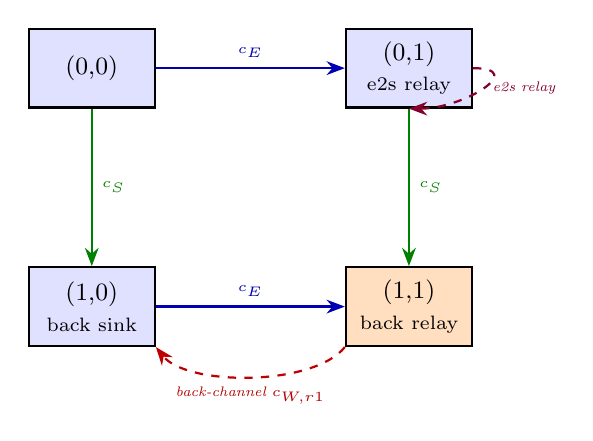
\begin{tikzpicture}[every node/.style={font=\footnotesize}]
  \node[pe,fill=blue!12]                  (p00) {(0,0)};
  \node[pe,fill=blue!12,right=2.4cm of p00] (p01) {(0,1)\\\scriptsize e2s relay};
  \node[pe,fill=blue!12,below=2.0cm of p00] (p10) {(1,0)\\\scriptsize back sink};
  \node[pe,fill=orange!25,below=2.0cm of p01] (p11) {(1,1)\\\scriptsize back relay};
  % Row data (east) on c_E
  \draw[source] (p00) -- node[above,font=\tiny]{$c_E$} (p01);
  \draw[source] (p10) -- node[above,font=\tiny]{$c_E$} (p11);
  % Col data (south) on c_S
  \draw[colsrc] (p00) -- node[right,font=\tiny]{$c_S$} (p10);
  \draw[colsrc] (p01) -- node[right,font=\tiny]{$c_S$} (p11);
  % Back-channel (row 1)
  \draw[backch] (p11.south west) ..controls +(-0.4,-0.5) and +(0.4,-0.5)..
        (p10.south east)
        node[midway,below,font=\tiny\itshape,red!70!black]
        {back-channel $c_{W,r1}$};
  % e2s relay (PE 0,1 forwards east arrivals onto south)
  \draw[->,>=Stealth,thick,purple!70!black,dashed]
        (p01.east) ..controls +(0.7,0) and +(0.7,0).. (p01.south)
        node[midway,right,font=\tiny\itshape] {e2s relay};
\end{tikzpicture}
\end{center}

\paragraph{Per-PE queues ($2 \times 2$).} Fits 6/6 by hardcoding
the topology to $2 \times 2$:

\begin{center}\footnotesize
\begin{tabular}{ll}
\toprule
PE (0,0) NW & 1 OQ east + 1 OQ south + barrier IQ/OQ row + barrier IQ/OQ col \\
PE (0,1) NE & 1 IQ east (recv c\_E) + 1 OQ south (e2s relay) + barriers \\
PE (1,0) SW & 1 IQ south + 1 IQ back-channel + 1 IQ east + barriers \\
PE (1,1) SE & 1 IQ east + 1 IQ south + 1 OQ back-channel + barriers \\
\bottomrule
\end{tabular}
\end{center}

But before going general, we made one detour first.

\subsection{\code{pipelined-lww 2d\_seg}, single-axis segmented in 2D namespace}
\textbf{Files:} \file{csl/layout\_lww\_2d\_seg.csl},
\file{csl/pe\_program\_lww\_2d\_seg.csl}.

While we were figuring out the right way to do dual-axis, we
needed a kernel that could at least scale 1D \emph{or} a single
column to many PEs in the 2D framework. \code{2d\_seg} is exactly
\code{east\_seg} lifted into the 2D namespace, with a small
twist: when the runner asks for $1 \times N$ the segmented
pipeline runs east; when it asks for $N \times 1$ the same
pipeline runs south. Internally the routes use a
direction-agnostic macro pair (\code{DIR\_IN}, \code{DIR\_OUT})
that resolves to \code{WEST/EAST} or \code{NORTH/SOUTH} based on
which axis is active. The kernel sees the active-axis length as
\code{num\_cols} regardless, so all the segment math is the same.

Color and queue counts are identical to \code{east\_seg}. The
only new thing this kernel does is \emph{handle either axis with
one codebase}. Validated up to $1 \times 16$ and $16 \times 1$.

This kernel is still in active use, when someone asks for
$1 \times N$ or $N \times 1$ today via
\code{--lww-layout 2d\_seg2}, the layout file detects the
single-axis case and dispatches \emph{this} kernel under the
hood. So \code{2d\_seg} is the stable 1D backbone underneath the
dual-axis kernel.

\paragraph{Layout sketch.} Same colors and queues as
\code{east\_seg} but the layout file picks the active axis at
compile time. When \code{num\_rows == 1}, the segmented pipeline
runs east. When \code{num\_cols == 1}, the same pipeline rotates
ninety degrees and runs south.

\begin{center}
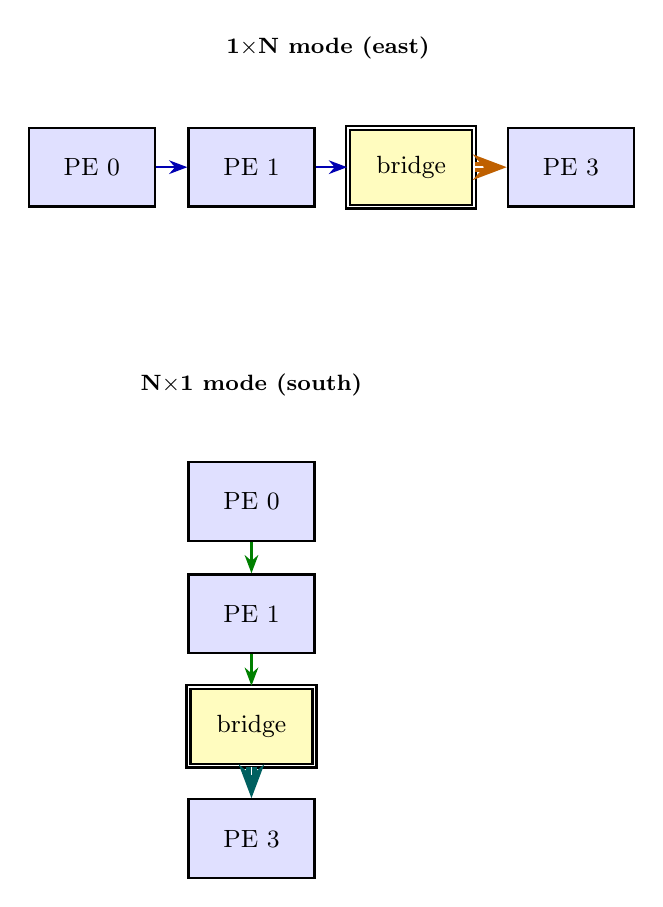
\begin{tikzpicture}[every node/.style={font=\footnotesize},node distance=0.4cm]
  \node[align=center] {\textbf{1$\times$N mode (east)}};
  \node[pe,fill=blue!12,below=1.0cm,xshift=-3.0cm] (a0) {PE 0};
  \node[pe,fill=blue!12,right=of a0] (a1) {PE 1};
  \node[pebridge,right=of a1]        (a2) {bridge};
  \node[pe,fill=blue!12,right=of a2] (a3) {PE 3};
  \draw[source] (a0) -- (a1);
  \draw[source] (a1) -- (a2);
  \draw[bridge] (a2) -- (a3);
  % south mode below
  \node[align=center,below=2.5cm of a1.center] (lab2) {\textbf{N$\times$1 mode (south)}};
  \node[pe,fill=blue!12,below=0.7cm of lab2.south] (b0) {PE 0};
  \node[pe,fill=blue!12,below=of b0] (b1) {PE 1};
  \node[pebridge,below=of b1]        (b2) {bridge};
  \node[pe,fill=blue!12,below=of b2] (b3) {PE 3};
  \draw[colsrc] (b0) -- (b1);
  \draw[colsrc] (b1) -- (b2);
  \draw[colbridge] (b2) -- (b3);
\end{tikzpicture}
\end{center}

\paragraph{Per-PE queues.} Identical to \code{east\_seg}: 9
colors total, 6 queues used at the bridge PE, fewer elsewhere.
The runner enforces that exactly one of \code{num\_rows} or
\code{num\_cols} equals 1 for this layout.

\subsection{\code{pipelined-lww 2d\_seg2}. Composing everything for any grid}
\textbf{Files:} \file{csl/layout\_lww\_2d\_seg2.csl},
\file{csl/pe\_program\_lww\_2d\_seg2.csl}.

This is the kernel where everything we learned came together.
The goal was simple in words. \textbf{Run dual-axis at any grid
size from 2 by 2 to as big as the fabric permits, with one
fixed compiled binary.} We pin the segment size at $S = 2$, so
each segment is two PEs wide on each axis, and we stack every
trick we have learned. There are five pieces:

\begin{enumerate}[leftmargin=1.3em,itemsep=0.15em]
  \item Segment plus bridge on the row axis, exactly as in
    \code{east\_seg}. Source colors are \code{c\_0} and
    \code{c\_1}. Bridge colors are \code{c\_be} and
    \code{c\_bo}.
  \item Segment plus bridge on the column axis, the mirror
    image of the row axis. Source colors are \code{c\_col\_0}
    and \code{c\_col\_1}. Bridge colors are \code{c\_col\_be}
    and \code{c\_col\_bo}.
  \item The east-to-south relay, generalized. In the old
    \code{2d} kernel only row 0 had this relay. Now any PE with
    \code{col > 0} re-emits east arrivals onto its south
    stream.
  \item The per-row back-channel, generalized. In the old
    \code{2d} kernel only row 1 had a back-channel. Now every
    row above row 0 has its own westbound back-channel that
    runs from the east-edge column toward column 0. The
    back-channel carries the south-west anti-diagonal wavelets
    that the rest of the topology cannot reach.
  \item The alternating reduce chain on each axis. This is the
    same \code{sync\_reduce\_c0} and \code{sync\_reduce\_c1}
    pattern we have used since the 1D kernel, replicated on
    rows and columns.
\end{enumerate}

Here is what the layout looks like at 4 by 4:

\begin{center}
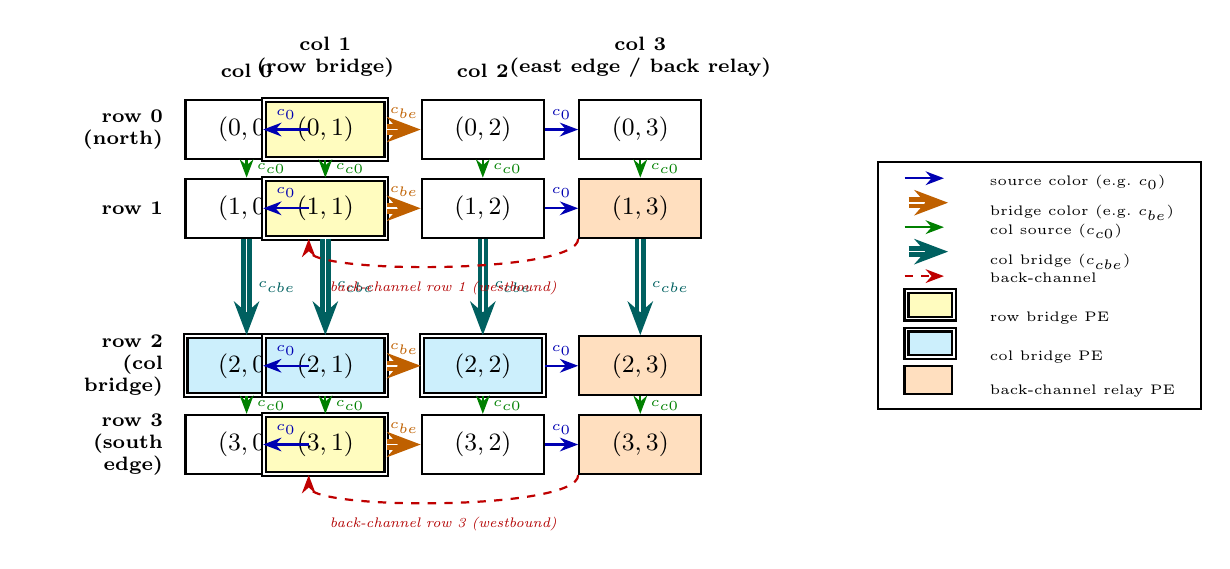
\begin{tikzpicture}[every node/.style={font=\scriptsize},
                    pe/.append style={minimum width=1.55cm,minimum height=0.75cm},
                    >=Stealth]
  % --- 4x4 grid of PEs ---
  \foreach \r in {0,1,2,3} {
    \foreach \c in {0,1,2,3} {
      \pgfmathtruncatemacro\rowy{-\r*1.6}
      \pgfmathtruncatemacro\colx{\c*1.85}
      % Choose styling per role
      \ifnum\c=1 \def\style{pebridge}\else\ifnum\c=3 \def\style{pe}\else\def\style{pe}\fi\fi
      \ifnum\r=2 \def\style{pecolbridge}\fi
      \ifnum\r>0 \ifnum\c=3 \def\style{pebackrelay}\fi\fi
      \ifnum\r=1 \ifnum\c=1 \def\style{pebridge}\fi\fi
      \ifnum\r=3 \ifnum\c=1 \def\style{pebridge}\fi\fi
      \node[\style] (p\r\c) at (\colx,\rowy) {$(\r,\c)$};
    }
  }
  % --- Row data arrows (east-going) ---
  \foreach \r in {0,1,2,3} {
    \draw[source] (p\r0.east) -- node[above,font=\tiny]{$c_0$} (p\r1.west);
    \draw[bridge] (p\r1.east) -- node[above,font=\tiny]{$c_{be}$} (p\r2.west);
    \draw[source] (p\r2.east) -- node[above,font=\tiny]{$c_0$} (p\r3.west);
  }
  % --- Col data arrows (south-going) ---
  \foreach \c in {0,1,2,3} {
    \draw[colsrc]    (p0\c.south) -- node[right,font=\tiny]{$c_{c0}$} (p1\c.north);
    \draw[colbridge] (p1\c.south) -- node[right,font=\tiny]{$c_{cbe}$} (p2\c.north);
    \draw[colsrc]    (p2\c.south) -- node[right,font=\tiny]{$c_{c0}$} (p3\c.north);
  }
  % --- Back-channel for row 1 and row 3 (westbound) ---
  \draw[backch] (p13.south west) ..controls ($(p13.south west)+(0,-0.45)$) and
                                 ($(p10.south east)+(0,-0.45)$) ..
                (p10.south east)
       node[midway,below=2pt,font=\tiny\itshape,red!70!black]
       {back-channel row 1 (westbound)};
  \draw[backch] (p33.south west) ..controls ($(p33.south west)+(0,-0.45)$) and
                                 ($(p30.south east)+(0,-0.45)$) ..
                (p30.south east)
       node[midway,below=2pt,font=\tiny\itshape,red!70!black]
       {back-channel row 3 (westbound)};
  % --- Column header labels ---
  \foreach \c/\lab in {0/{col 0},1/{col 1\\(row bridge)},2/{col 2},3/{col 3\\(east edge / back relay)}} {
    \node[align=center,font=\scriptsize\bfseries,above=0.15cm of p0\c] {\lab};
  }
  % --- Row header labels ---
  \foreach \r/\lab in {0/{row 0\\(north)},1/{row 1},2/{row 2\\(col bridge)},3/{row 3\\(south edge)}} {
    \node[align=right,font=\scriptsize\bfseries,left=0.15cm of p\r0,text width=1.6cm] {\lab};
  }
  % --- Legend ---
  \node[draw,thick,fill=white,align=left,font=\tiny,
        anchor=north west] (leg) at (8.0,-0.4) {
    \begin{tabular}{ll}
      \tikz\draw[source] (0,0) -- (0.5,0); & source color (e.g.\ $c_0$) \\
      \tikz\draw[bridge] (0,0) -- (0.5,0); & bridge color (e.g.\ $c_{be}$) \\
      \tikz\draw[colsrc] (0,0) -- (0.5,0); & col source ($c_{c0}$) \\
      \tikz\draw[colbridge] (0,0) -- (0.5,0); & col bridge ($c_{cbe}$) \\
      \tikz\draw[backch] (0,0) -- (0.5,0); & back-channel \\
      \tikz\node[pebridge,minimum width=0.6cm,minimum height=0.35cm]{}; & row bridge PE \\
      \tikz\node[pecolbridge,minimum width=0.6cm,minimum height=0.35cm]{}; & col bridge PE \\
      \tikz\node[pebackrelay,minimum width=0.6cm,minimum height=0.35cm]{}; & back-channel relay PE \\
    \end{tabular}};
\end{tikzpicture}
\end{center}

Things to notice in that picture:

\begin{itemize}[leftmargin=1.3em,itemsep=0.1em]
  \item The row of PEs across the top is just like our 1D
    \code{east\_seg} kernel, with source colors and a bridge
    column at position 1.
  \item The same pattern repeats vertically. Columns have their
    own source colors \code{c\_col\_0} and \code{c\_col\_1} and
    their own bridge colors \code{c\_col\_be} and
    \code{c\_col\_bo}. Row 2 in this picture is a column-bridge
    row.
  \item For every row above row 0, the rightmost PE (the back
    relay) sends a westbound back-channel toward column 0. The
    back-channel carries the wavelets that originated north and
    east of the receiver but need to reach a south-west
    receiver.
\end{itemize}

Putting all five pieces together gives us a working dual-axis
kernel. Unfortunately it also blows the 6-queue budget at the
hardest-working PEs. At a fully interior bridge PE (one that is
a bridge on both axes) we counted seven or eight distinct input
queues needed. We had to fix that. We did it in a sequence of
three checkpoints that we named CP2d.c, CP2d.d.1, and
CP2d.d.2. Each one collapsed one stream into another by adding
a few opcode bits to the wavelet header.

\paragraph{CP2d.c.} We moved the column broadcast in-band onto
the south data stream. We used a bit-29 opcode flag, exactly
the same trick the old \code{2d} kernel had used for the row
broadcast on the east data stream. Now there is no separate
\code{col\_bcast\_recv} input queue. The south data input
queue handles both data wavelets and broadcast wavelets, and
the receiver task tells them apart by looking at bit 29. We
freed one input queue.

\paragraph{CP2d.d.1.} We did the same thing for the row
broadcast on the east data stream. One more input queue freed.
We also got back one output queue (the dedicated row broadcast
OQ).

\paragraph{CP2d.d.2.} This one was the real breakthrough. We
folded the entire back-channel onto the existing row reduce
chain. Before this checkpoint, the back-channel had its own
dedicated color and its own input queue at every interior PE.
The reduce chain already had exactly the right shape for what
the back-channel needed (an east-edge initiator, alternating
colors through the row, a west-edge consumer). So we let
back-channel data wavelets ride the same colors as the reduce
wavelets, distinguished by a second opcode bit, bit 28. The
receiver task at each chain PE looks at bit 28. If it is a
reduce wavelet, the task does the OR-and-forward step. If it
is a back-channel data wavelet, the task hands it to the
south-data handler and re-emits it westward on the same chain.

After CP2d.d.2 the interior-interior PE queue map locks at six
out of six \textbf{for any grid size at $S = 2$}. The exact
mapping looks like this:

\begin{center}
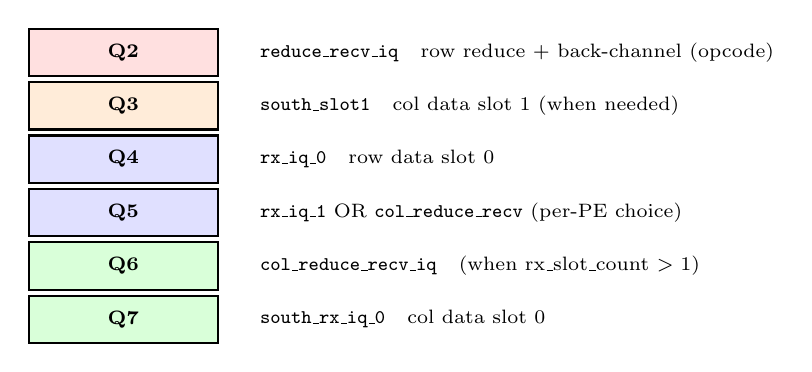
\begin{tikzpicture}[node distance=0.05cm,
                    qbox/.style={draw,thick,minimum width=2.4cm,minimum height=0.6cm,
                                 align=center,font=\scriptsize}]
  \node[qbox,fill=red!12]    (q2) {\textbf{Q2}};
  \node[qbox,fill=orange!15,below=of q2] (q3) {\textbf{Q3}};
  \node[qbox,fill=blue!12,below=of q3]   (q4) {\textbf{Q4}};
  \node[qbox,fill=blue!12,below=of q4]   (q5) {\textbf{Q5}};
  \node[qbox,fill=green!15,below=of q5]  (q6) {\textbf{Q6}};
  \node[qbox,fill=green!15,below=of q6]  (q7) {\textbf{Q7}};
  \node[right=0.4cm of q2,font=\scriptsize,anchor=west]
    {\code{reduce\_recv\_iq}\quad row reduce + back-channel (opcode)};
  \node[right=0.4cm of q3,font=\scriptsize,anchor=west]
    {\code{south\_slot1}\quad col data slot 1 (when needed)};
  \node[right=0.4cm of q4,font=\scriptsize,anchor=west]
    {\code{rx\_iq\_0}\quad row data slot 0};
  \node[right=0.4cm of q5,font=\scriptsize,anchor=west]
    {\code{rx\_iq\_1} OR \code{col\_reduce\_recv} (per-PE choice)};
  \node[right=0.4cm of q6,font=\scriptsize,anchor=west]
    {\code{col\_reduce\_recv\_iq}\quad (when rx\_slot\_count $> 1$)};
  \node[right=0.4cm of q7,font=\scriptsize,anchor=west]
    {\code{south\_rx\_iq\_0}\quad col data slot 0};
\end{tikzpicture}
\end{center}

Six input queues, all in use, no kind of mail dropped. The same
compiled binary now runs at 2 by 2, 4 by 4, 8 by 8, 16 by 16,
and 2 by 16. We have validated every one of these grid sizes.
Section~\ref{sec:timing-2d} has the cycle counts. From the
queue-cap and color-cap point of view there is nothing in the
way of the full WSE-3.

For a while we worried that the chain-merged back-channel
might run into output-queue backpressure on dense graphs. The
concern was that test12 (twenty-node graph at 8 by 8) would
push so many wavelets through \code{tx\_reduce\_oq} on each
chain PE that the CPU's \code{@mov32} would block waiting for
the fabric to drain. We even sketched a follow-up checkpoint,
CP2d.e, that would move the back-channel back onto its own
dedicated fabric-forwarded color. \textbf{In the latest rerun,
however, test12 at 8 by 8 PASSED}, with 5 levels and 952{,}663
cycles total. Whatever the earlier hang was, it appears to
have been resolved by the layout fixes that landed alongside
CP2d.d.2. We are keeping CP2d.e as a possible future
optimization rather than a required scaling fix.

\subsection{\code{pipelined-lww 2d\_multicast}, an orthogonal optimization}
\textbf{Files:} \file{csl/layout\_lww\_2d\_multicast.csl},
\file{csl/pe\_program\_lww\_2d\_multicast.csl}.

This kernel is not part of the scaling story; it is an
\emph{efficiency} sidequest layered on top of \code{2d} iter 2.
The observation: in our other kernels, when a local vertex has,
say, three graph neighbors that all happen to live on the same
downstream PE, we generate three identical wavelets, one per
boundary entry, even though one would have sufficed. That is
wasted bandwidth.

\code{2d\_multicast} fixes this by iterating \emph{local
vertices} instead of \emph{boundary entries} when packing the
send buffer, and consulting two bitmaps uploaded by the host:
\code{should\_send\_east[v]} and \code{should\_send\_south[v]}.
If a vertex has no boundary neighbor on the east axis, the
kernel just skips its east wavelet. If it has at least one but
all on the same downstream PE, one wavelet still goes out, but
only one.

This is a real perf win, but it inherits all the $2 \times 2$
shape limits of \code{2d} iter 2, it does not by itself
extend to larger grids. The deduplication idea would layer
cleanly on top of \code{2d\_seg2} if we ever bring the two
together.

\paragraph{Layout sketch.} Identical to \code{2d} iter 2 (same
fabric, same colors, same queues). The only change is at the
\emph{sender} CPU: it consults a host-uploaded bitmap before
emitting each wavelet. Same picture as \S3.5 with an extra
filter step at every PE's send path.

\begin{center}
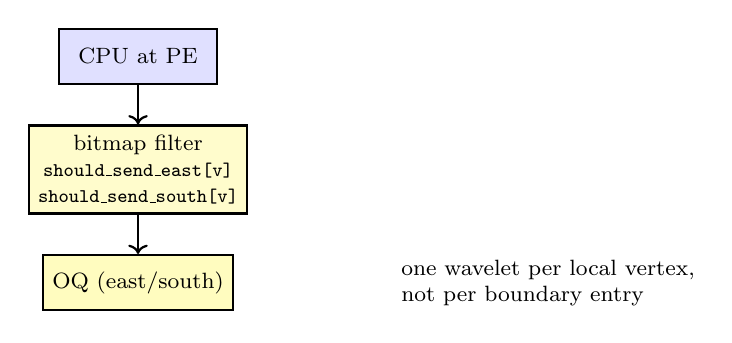
\begin{tikzpicture}[every node/.style={font=\footnotesize},node distance=0.5cm]
  \node[draw,thick,minimum width=2.0cm,minimum height=0.7cm,fill=blue!12]
        (cpu) {CPU at PE};
  \node[draw,thick,fill=yellow!20,below=of cpu,align=center,minimum width=2.4cm]
        (filter) {bitmap filter\\\scriptsize \code{should\_send\_east[v]}\\\scriptsize \code{should\_send\_south[v]}};
  \node[draw,thick,minimum width=2.0cm,minimum height=0.7cm,below=of filter,fill=yellow!25]
        (oq) {OQ (east/south)};
  \node[right=2.0cm of oq,align=left] {one wavelet per local vertex,\\not per boundary entry};
  \draw[->,thick] (cpu) -- (filter);
  \draw[->,thick] (filter) -- (oq);
\end{tikzpicture}
\end{center}

\subsection{\code{hw-filter}, the dead-end branch worth knowing about}
\textbf{Files:} \file{csl/layout\_hw\_broadcast.csl},
\file{csl/pe\_program\_hw\_broadcast.csl}.

For completeness: at one point we tried to use the WSE-3
hardware broadcast filter, a feature that lets the fabric
drop wavelets whose payload does not match a per-PE filter. The
idea was that we could send wavelets from a PE to \emph{all} its
downstream neighbors at once and let the hardware filter pick
out the right ones. The filter works for one-hop delivery, but
multi-hop would have required SW relay buffers we never built,
and the cap was around 5 PEs (1D only). Not worth pursuing once
\code{east\_seg} was working. We keep the kernel around for
reference.

\paragraph{Layout sketch (1D, 4 PEs, HW broadcast filter).}
Four-color checkerboard, exactly like \code{sw-relay} except
the fabric switches drop wavelets whose payload does not match
the receiver's filter. One-hop only.

\begin{center}
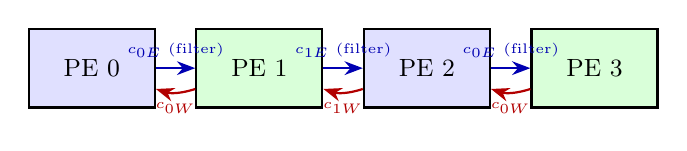
\begin{tikzpicture}[every node/.style={font=\footnotesize},node distance=0.5cm]
  \node[pe,fill=blue!12]              (p0) {PE 0};
  \node[pe,fill=green!15,right=of p0] (p1) {PE 1};
  \node[pe,fill=blue!12,right=of p1]  (p2) {PE 2};
  \node[pe,fill=green!15,right=of p2] (p3) {PE 3};
  \draw[source] (p0) -- node[above,font=\tiny]{$c_{0E}$ (filter)} (p1);
  \draw[source] (p1) -- node[above,font=\tiny]{$c_{1E}$ (filter)} (p2);
  \draw[source] (p2) -- node[above,font=\tiny]{$c_{0E}$ (filter)} (p3);
  \draw[->,>=Stealth,thick,red!70!black] (p1) to[bend left=18]
        node[below,font=\tiny]{$c_{0W}$} (p0);
  \draw[->,>=Stealth,thick,red!70!black] (p2) to[bend left=18]
        node[below,font=\tiny]{$c_{1W}$} (p1);
  \draw[->,>=Stealth,thick,red!70!black] (p3) to[bend left=18]
        node[below,font=\tiny]{$c_{0W}$} (p2);
\end{tikzpicture}
\end{center}

\paragraph{Per-PE queues.}
2 IQ + 2 OQ data + barrier IQ/OQ, inside the cap. The fabric
switch's HW filter takes care of dropping non-matching
wavelets, so the CPU only ever sees relevant ones.

\section{WSE-3 architectural limitations that shaped the design}
\label{sec:overcome}

\subsection{Six-queue-per-PE cap (hard)}
WSE-3 exposes 6 user input queues and 6 user output queues per PE
(queues 2--7; 0--1 are reserved). Every fabric color the CPU
receives consumes one IQ; every color it emits consumes one OQ.
Multiple colors cannot share a queue.

\textbf{Impact.} A naive 2D kernel needs $2$ row-data slots $+\,2$
col-data slots $+\,$row-reduce-recv $+\,$row-bcast-recv
$+\,$col-reduce-recv $+\,$col-bcast-recv $+\,$back-channel-recv
$\approx 8$ IQs. Over-budget.

\subsection{Single rx-direction per color (hard on WSE-3)}
A fabric color's route at each PE accepts wavelets from \emph{at
most one} direction (\code{RAMP}, \code{EAST}, \code{WEST},
\code{NORTH}, \code{SOUTH}). \code{tx} can be multiple. CSL
enforces this on WSE-3 with the error
\code{expected at most 1 input direction(s) on 'wse3', got: 2}.

\textbf{Impact.} A single color cannot both accept CPU-injected
wavelets (\code{rx=RAMP}) \emph{and} forward fabric arrivals
(\code{rx=EAST}). Accumulating chains require
\textbf{two alternating colors per axis} with OR-at-CPU between
hops.

\subsection{CP3: same-color inject + non-RAMP rx is silently dropped}
If a PE's CPU emits on color $X$ while the color's route has
\code{rx} from a fabric direction (not RAMP), the injected wavelet
is silently dropped on WSE-3, no compile error, no runtime
fault. Forbids fan-in patterns where every PE injects its own
bit on a shared color.

\subsection{One OQ = one color}
Binding an OQ to color $A$ and emitting with
\code{fabric\_color = $B$} is a runtime fault that surfaces as a
kernel stall (host-side timeout, \code{std::runtime\_error: received
length 0}). Discovered 2026-04-21 in
\file{csl/pe\_program\_lww\_2d.csl} iter 1.

\textbf{Impact.} Two stream types on disjoint colors require two
OQs. Combining them in-band on the same color via opcode bits
avoids the OQ inflation, this is how we moved
\code{row\_bcast}, \code{col\_bcast}, and eventually back-channel
data in-band.

\subsection{Finite fabric-color budget ($\sim 24$ usable)}
WSE-3 has 32 colors total; after \code{memcpy} reservations and
the three fixed barrier colors we target, roughly 24 are usable
for data-plane plumbing. A per-PE-dedicated color scheme does
not scale.

\subsection{OQ depth is small ($\sim 32$ wavelets), backpressures without deadlock}
Each OQ buffers a small number of wavelets. Pushing more than it
can hold blocks the CPU at \code{@mov32} until the fabric drains.
Under heavy load, a chain where every PE re-emits every wavelet
through its own OQ saturates quickly. Not a correctness bug, but a
performance cliff (observed at $8\times 8$ test12 under
\code{2d\_seg2}, see Section~\ref{sec:backpressure}).

\subsection{Monotone ID vs. geometry mismatch}
Path C assigns contiguous GID ranges in row-major PE order so the
invariant
\[
\mathrm{gid}_a < \mathrm{gid}_b \;\Rightarrow\;
\mathrm{pe}(\mathrm{gid}_a) \le \mathrm{pe}(\mathrm{gid}_b)
\]
holds. Under ``lower-GID wins,'' the eastern / southern PE always
loses. On the col axis (and the anti-diagonal SW class) the loser
sits south-west, fabric data flows north-south and west-east,
so we reach SW receivers via a \emph{back-channel}
(PE$(R, \mathrm{last\_col}) \to$ westward chain).

\section{How we overcame each limitation}

\subsection{Queue-cap collapse via in-band opcodes}
Rather than allocate a distinct color per stream type, we pack
stream-discriminator bits into the 32-bit wavelet and dispatch
on arrival:

\begin{lstlisting}
Data:          [31]=0, [30]=parity, [29:8]=gid, [7:0]=color
Data-done:     [31]=1, [30]=parity, [29]=0, [28]=0
Row/col bcast: [31]=1, [30]=parity, [29]=1, [0]=value
Row-reduce:    [31]=1, [30]=parity, [29]=0, [28]=1, [0]=value
\end{lstlisting}

The receiver task (\code{reduce\_recv\_task} in
\file{csl/pe\_program\_lww\_2d\_seg2.csl}) decodes and dispatches.
Each opcode merge frees one IQ + one OQ: CP2d.c folded
\code{col\_bcast} onto the south data stream, CP2d.d.1 folded
\code{row\_bcast} onto the east data stream, CP2d.d.2 folded
back-channel data onto the row-reduce chain.

\paragraph{Interior-interior PE queue map at $S=2$ after CP2d.d.2:}
\begin{center}
\begin{tabular}{cl}
\toprule
Q & IQ role \\
\midrule
Q2 & \code{reduce\_recv\_iq} (row\_reduce + back-channel via opcode) \\
Q3 & \code{south\_slot1} (conditional on rx\_slot\_count / cy\_is\_south / num\_cols) \\
Q4 & \code{rx\_iq\_0} (row data slot 0) \\
Q5 & \code{rx\_iq\_1} OR \code{col\_reduce\_recv} OR \code{south\_slot1} (per-PE) \\
Q6 & \code{col\_reduce\_recv\_iq} (when rx\_slot\_count $> 1$) \\
Q7 & \code{south\_rx\_iq\_0} (col data slot 0) \\
\bottomrule
\end{tabular}
\end{center}

$6/6$, $N$-invariant at $S=2$.

\subsection{Color reuse via bridges (CP2a pattern, generalized to 2D)}
Per-PE-dedicated colors would saturate the $\sim\!24$-color budget
at $\mathrm{num\_cols} > 5$. We avoid this with \textbf{span-
disjoint reuse}:

\begin{itemize}[leftmargin=1.1em,itemsep=0.2em]
  \item \textbf{Source colors} $c_0 \ldots c_{S-1}$ (and
    $c\_col_0 \ldots c\_col_{S-1}$) are local to each segment of
    length $S$. PE at $\mathrm{local\_x}=j$ injects on $c_j$;
    downstream PEs in the same segment receive; the color dies at
    the segment's bridge. Reused in the next segment.
  \item \textbf{Bridge colors} alternate by segment index:
    $c_{be}$ for $\mathrm{seg\_idx}$ even, $c_{bo}$ for odd.
    Bridge $k$ terminates at bridge $k{+}1$, so reuse two segments
    later is safe.
  \item \textbf{Back-channel / reduce colors} reuse by row parity
    ($c\_W\_back\_re$ even rows, $c\_W\_back\_ro$ odd).
\end{itemize}

Total fabric-color count stays near 10--12 regardless of grid size.

\subsection{Single-rx constraint $\to$ alternating-chain reduce}
Because we cannot do \code{rx=\{EAST, RAMP\}} on one color, the
row\_reduce chain uses two colors, alternating per-PE parity:

\begin{lstlisting}
PE(R, k) even col:  recv on sync_reduce_c0 (rx=EAST tx=RAMP)
                    send on sync_reduce_c1 (rx=RAMP tx=WEST)
PE(R, k) odd col:   recv on sync_reduce_c1
                    send on sync_reduce_c0
\end{lstlisting}

CPU at each interior PE OR's the incoming reduce value with its
local \code{has\_uncolored} bit and re-emits westward. Terminus
PE$(R, 0)$ broadcasts the result east (row\_bcast). The same
alternating chain now ferries back-channel data via opcode bits.

\subsection{CP3 prohibition $\to$ CPU-mediated re-injection}
Anywhere we want a wavelet to change color mid-route (segment
bridges, e2s anti-diagonal relay), we do it via CPU:
\code{bridge\_reinject} and \code{col\_bridge\_reinject} in
\file{csl/pe\_program\_lww\_2d\_seg2.csl} receive the wavelet at
RAMP and re-emit on a different color. Slower than a fabric
forward, but legal.

\subsection{Anti-diagonal SW delivery $\to$ per-row back-channel}
Under Path C, some cross-PE conflicts have winner in column $C_1$
and loser in column $C_2 < C_1$ of a row below. We reach them via:

\begin{enumerate}[leftmargin=1.3em,itemsep=0.2em]
  \item PE$(R_w, C_1)$ sends south on $c\_col\_\ast$.
  \item At PE$(R_l, C_1)$, the south stream hits a relay that is
    also a back-channel source (\code{is\_back\_relay}: east-edge
    column for row $> 0$).
  \item That PE forwards the wavelet westward on the back-channel
    (folded onto the reduce chain).
  \item Every PE between $C_1$ and $C_2$ also gets a RAMP copy
    via the CPU tap, so interior SW receivers see the winner.
\end{enumerate}

\subsection{OQ-depth backpressure, acknowledged, CP2d.e pending}
\label{sec:backpressure}
Dense graphs at $8\times 8$ trigger $\sim\!\mathrm{row}\cdot
\mathrm{num\_cols}$ back-channel wavelets per round that all route
through the CPU-mediated chain on \code{tx\_reduce\_oq}. Under
saturation we stall. The planned mitigation (CP2d.e,
Section~\ref{sec:cp2de}) restores a fabric-forwarded back-channel
route on a freed queue, keeping the merge only for row\_reduce.

\section{How the algorithm fits the hardware}

Picasso's level-$L$ loop is a BSP:

\begin{enumerate}[leftmargin=1.3em,itemsep=0.2em]
  \item \textbf{Speculate}, each PE picks a tentative color
    respecting its local and remote colors.
  \item \textbf{Exchange}, each PE sends tentative colors to
    boundary neighbors. The pipelined-LWW transport serves this
    phase: per-boundary east / south / back-channel wavelets.
  \item \textbf{Detect + resolve}, compare local and received
    colors at shared boundaries; if they match, the higher-GID PE
    reverts to $-1$. Under Path C, always the eastern or southern
    PE.
  \item \textbf{Barrier}, global OR-reduce of
    \code{has\_uncolored}. Round done iff zero; else next round.
    Row-reduce + col-reduce chains + bcasts implement this.
\end{enumerate}

Key architectural fits:

\begin{itemize}[leftmargin=1.3em,itemsep=0.2em]
  \item \textbf{Round-parity tagging} (\code{[30]=parity}) lets
    fast PEs send round $k{+}1$ wavelets before slow PEs finish
    round $k$; staging buffers promote next-round wavelets at
    \code{reset\_round\_state}.
  \item \textbf{Bridges and alternating reduce} are both direct
    consequences of the single-rx constraint.
  \item \textbf{Monotone block partition (Path C)} turns the
    conflict-loser rule into a fabric-direction rule (east /
    south loses), which drives the entire east $+$ south $+$
    SW-back-channel topology.
\end{itemize}

The algorithm needed essentially no change; only the transport
evolved.

\section{Timing data collected so far (simulator, WSE-3 arch)}

\subsection{Small-grid comparison (1D 4-PE, all 13 tests)}
\label{sec:timing-1d}

Total cycles across all levels. Source:
\file{LWW\_PICASSO\_RESULTS.md}.

\begin{center}
\begin{tabular}{l r r r}
\toprule
Test & SW-relay (cyc) & LWW east\_seg (cyc) & Speedup \\
\midrule
test1 & 30,801 & 21,889 & $1.41\times$ \\
test2 & 13,067 & 10,211 & $1.28\times$ \\
test3 & 39,272 & 29,547 & $1.33\times$ \\
test5 & 71,747 & 53,974 & $1.33\times$ \\
test6 & 214,684 & 179,222 & $1.20\times$ \\
test7 & 360,849 & 326,376 & $1.11\times$ \\
test10 & 34,365 & 27,614 & $1.24\times$ \\
\bottomrule
\end{tabular}
\end{center}

\subsection{Dual-axis 2d\_seg2 timings (new, 2026-04-24)}
\label{sec:timing-2d}

Total cycles across all levels per test. Not strictly comparable
across grid sizes because \code{expected\_data\_done} grows with
$N$ and graphs distribute differently.

\begin{center}
\begin{tabular}{l l r r l}
\toprule
Grid & Test & Levels & Cycles & Source \\
\midrule
$4\times 4$ & test1 & 2 & 12,176 & v4 regression \\
$4\times 4$ & test3 & 2 & 27,572 & v4 regression \\
$4\times 4$ & test10 & 2 & 33,626 & v4 regression \\
$4\times 4$ & test11 & 5 & 276,621 & v4 regression \\
$4\times 4$ & test12 & 5 & 740,376 & v4 regression \\
$4\times 4$ & test7 & 3 & 220,016 & v4 regression \\
$8\times 8$ & test1 & 2 & 66,635 & v7 sparse \\
$8\times 8$ & test3 & 2 & 72,186 & sparse \\
$8\times 8$ & test12 (dense, 20 nodes) & 5 & 952{,}663 (1.12 ms) & rerun PASS \\
$16\times 16$ & test1 & 2 & 252,317 & sparse \\
$2\times 16$ & test1 & 2 & 41,875 & rectangular \\
\bottomrule
\end{tabular}
\end{center}

Source directories under
\file{runs/local/20260424-2d-seg2-*-cp2dd2*}.

\textbf{Read-outs.} Cycle cost scales roughly linearly with grid
diameter ($16\times 16$ test1 $\approx 3.8\times$ of $8\times 8$
test1), consistent with the $O(\mathrm{rows} + \mathrm{cols})$
barrier chain for sparse graphs. $2\times 16$ is cheaper than
$2\times 2$-denser graphs because test1 has little cross-PE
traffic. Dense-graph blow-up at $4\times 4$ (test12: 740k cyc, 5
levels) is real but completes; at $8\times 8$ the same graph
saturates the back-channel OQ (pending CP2d.e).

\subsection{What we are still missing}
\begin{itemize}[leftmargin=1.3em,itemsep=0.2em]
  \item No CS-3 hardware runs for \code{2d\_seg2} past $4\times 4$.
  \item No timing for $16\times 16$ dense tests (simulator is
    slow at 64+ PEs with dense graphs).
  \item No apples-to-apples SW-relay baseline at $\ge 8\times 8$
    for comparison.
\end{itemize}

\section{Plan}

\subsection{Bigger simulator test cases}
Goal: drive $8\times 8$ and $16\times 16$ to 13/13 on reasonable
graph sizes and record timing.

\begin{enumerate}[leftmargin=1.3em,itemsep=0.2em]
  \item Unblock $8\times 8$ dense (CP2d.e,
    Section~\ref{sec:cp2de}). Without this, test11, 12, 7 stall
    past level 0.
  \item Fresh batch runs, isolated per test to dodge the
    simulator regression-mode flake:

\begin{lstlisting}
for t in $(seq 1 13); do
  python3 picasso/run_csl_tests.py \
    --routing pipelined-lww --lww-layout 2d_seg2 \
    --num-pes 64 --grid-rows 8 --test testN_... \
    --run-id $(date +%Y%m%d)-2d-seg2-8x8-t${t}
done
\end{lstlisting}

    Same pattern at $16\times 16$. Persist each stdout under
    \file{runs/local/} for month-over-month diffs.
  \item Extend \file{LWW\_PICASSO\_RESULTS.md} with a new section
    per grid ($4\times 4$, $8\times 8$, $16\times 16$) showing
    total cycles, per-level cycles, rounds per level.
  \item Plot rounds $\times$ cycles-per-round vs. $N$ to see
    which axis dominates: more rounds (algorithm-bound) vs. more
    cycles per round (transport-bound).
\end{enumerate}

\subsection{CS-3 hardware runs (real WSE-3)}
The appliance path (\file{neocortex/run\_cs3.sh},
\file{run\_cs3\_batch.sh}) talks to a real CS-3 through
\code{SdkLauncher}. Same binary as simulator.

\begin{enumerate}[leftmargin=1.3em,itemsep=0.2em]
  \item Small set (test1, test5, test12) at $4\times 4$ through
    \file{run\_cs3.sh}. Validates the binary on real silicon.
  \item If $4\times 4$ is green on HW, scale to $8\times 8$.
    Simulator's dense-graph cliff at $8\times 8$ may not occur on
    real HW because OQ drain rate is much higher, a data
    point we genuinely lack.
  \item Compare HW timing to simulator cycle counts.
\end{enumerate}

\subsection{CP2d.e, dense-graph scaling fix}
\label{sec:cp2de}
Restore a dedicated \textbf{fabric-forwarded} back-channel route
(CP2d.c-style: \code{rx=EAST tx=\{WEST, RAMP\}}) on a freed queue
(Q6 where \code{col\_reduce\_recv} fits on Q5; Q3 otherwise). The
fabric switch auto-forwards westward at every interior PE.
no CPU \code{@mov32}, no OQ backpressure. Keep the reduce chain
on \code{sync\_reduce\_c0/c1} with opcode dispatch for row\_reduce
only.

Acceptance: $8\times 8$ test12 completes; $4\times 4$ 13/13 stays
green.

\subsection{On-device recursion feasibility}
Picasso is inherently recursive: each level prunes colored
vertices, then the uncolored subgraph is recolored with a smaller
palette. Today the recursion is \textbf{host-driven}, the
runner hands back per-level colorings, builds the next subgraph,
re-invokes the kernel. That is roughly 1 ms host-device RTT per
level, dominated by the coloring itself at current test sizes,
but potentially a floor at WSE-3 scale.

\textbf{Which kernels can accommodate on-device recursion?}

\begin{center}
\begin{tabular}{p{3.2cm} p{3.0cm} p{7.2cm}}
\toprule
Kernel & Can loop on device? & Why / obstacles \\
\midrule
\code{sw-relay} & Yes, but pointless & Each PE independent; trivial to loop but no speedup (SW relay is the bottleneck). \\
\code{pipelined-lww east\_seg} & Yes, with kernel changes & Ring-buffered boundary state, per-level re-entry. Needs on-device palette shrinkage, per-PE live-vertex mask, in-kernel level-done $\to$ level-begin transition. \\
\code{pipelined-lww 2d\_seg2} & Yes, same plan as \code{east\_seg} & Barrier + reduce primitives already exist. Main change: reset \code{remote\_recv\_color\_next}, data-done next-round counters, and fan-in residuals at level transitions. \\
\code{2d\_multicast} & Unclear & Fabric-switch-heavy; teardown + re-init between levels may be costly. Not the priority. \\
\bottomrule
\end{tabular}
\end{center}

The practical blocker is not the kernel, it is the data path for
\emph{palette changes}. Each level uses a smaller palette; the
kernel currently reads \code{palette\_size} from
\code{runtime\_config} set by the host. An on-device loop needs a
per-level shrinkage step (or just decrement
\code{palette\_size} after every level, the simplest).

\textbf{Recommendation.} Once CP2d.e is green, add a small
``level controller'' local task to \code{2d\_seg2} that gates
between levels: at barrier done, if \code{remaining > 0},
decrement \code{palette\_size}, call \code{reset\_round\_state},
\code{speculate\_task\_id}, and loop. Saves one host RTT per
level. At $8\times 8$ with roughly 5 rounds / level and 5 levels
on test12, that is $\sim 25$ round-trips removed, potentially
meaningful at real scale.

\subsection{Diagnose the 4$\times$4 / 2$\times$2 regression-mode flake}
The same test sometimes passes in isolation but hangs at level
$N \ge 1$ when run as part of \code{--test-range 1-13}. Single-
test \code{cerebras\_host.py} invocations are fresh Python
subprocesses, each spinning up its own simulator, so kernel state
cannot accumulate. The hang is simulator-process-accumulation or
a runner-side race.

\begin{enumerate}[leftmargin=1.3em,itemsep=0.2em]
  \item Reproduce under \code{strace} to see whether a subprocess
    is stuck on IPC or not exiting.
  \item Check whether repeated \code{cslc} invocations leak
    anything in \file{csl\_compiled\_out/} that a later test
    reads.
  \item Insert a \code{sleep 1} between tests and see whether
    the flake vanishes.
\end{enumerate}

Not blocking, the architecture is proven.

\section{Open questions}

\begin{itemize}[leftmargin=1.3em,itemsep=0.3em]
  \item $S=2$ forever, or grow to $S=4$? $S=4$ halves segment
    count (fewer bridges, fewer CPU reinjects) but needs 4 row
    data slots and pushes the queue budget over 6. Keep $S=2$
    for WSE-3 unless there is a specific perf reason.
  \item Host-driven vs on-device recursion, see previous
    section. Host-driven is simpler and debuggable; on-device is
    faster at large $N$.
  \item Partition quality (Step 5): hub clustering under naive
    block hurts test12 cycles by $\sim 50\%$; a degree-aware
    within-PE renumbering fixes the imbalance. Host-only
    change; deferred until $8\times 8$ dense is unblocked.
  \item When do we actually move to CS-3 hardware? Once
    $8\times 8$ / $16\times 16$ are green in simulator, there is
    no more reason to stay local.
\end{itemize}

\section{File and run-artifact index}

\paragraph{Primary kernel files (active):}
\begin{itemize}[leftmargin=1.3em,itemsep=0.15em]
  \item \file{csl/pe\_program\_lww\_2d\_seg2.csl}, dual-axis kernel, CP2d.d.2
  \item \file{csl/layout\_lww\_2d\_seg2.csl}, dual-axis layout
  \item \file{csl/pe\_program\_lww\_east\_seg.csl},
    \file{csl/layout\_lww\_east\_seg.csl}, 1D stable path
\end{itemize}

\paragraph{Legacy / experimental:}
\begin{itemize}[leftmargin=1.3em,itemsep=0.15em]
  \item \file{csl/layout\_lww\_2d.csl}, \file{pe\_program\_lww\_2d.csl}.
    $2\times 2$ iter-2 (superseded)
  \item \file{csl/layout\_lww\_2d\_seg.csl}, \file{pe\_program\_lww\_2d\_seg.csl}
   , single-axis seg (still dispatched by \code{2d\_seg2} for
    $1\times N$ / $N\times 1$)
  \item \file{csl/layout\_lww\_2d\_multicast.csl}, multicast fabric, not the
    main path
\end{itemize}

\paragraph{Plan / state docs:}
\begin{itemize}[leftmargin=1.3em,itemsep=0.15em]
  \item \file{AGENTS.md}, repo guide, checkpoint history
  \item \file{CURRENT\_STATE.md}, latest status
  \item \file{LWW\_PIPELINE\_PLAN.md}, detailed checkpoint plan / diffs
  \item \file{LWW\_PICASSO\_RESULTS.md}, original 1D 4-PE benchmark
  \item \file{WSE3\_SCALING\_ANALYSIS.md}, Markdown twin of this document
\end{itemize}

\paragraph{Recent run artifacts (CP2d.d validation, 2026-04-24):}
\begin{itemize}[leftmargin=1.3em,itemsep=0.15em]
  \item \file{runs/local/20260424-2d-seg2-4x4-tests1-13-cp2dd2-v4/}.
    $4\times 4$ 13/13 PASS
  \item \file{runs/local/20260424-2d-seg2-8x8-test1-cp2dd2/}.
    $8\times 8$ sparse PASS
  \item \file{runs/local/20260424-2d-seg2-8x8-test3-cp2dd2/}.
    $8\times 8$ anti-diagonal PASS
  \item \file{runs/local/20260424-2d-seg2-16x16-test1-cp2dd2/}.
    $16\times 16$ sparse PASS
  \item \file{runs/local/20260424-2d-seg2-2x16-test1-cp2dd2/}.
    rectangular PASS
\end{itemize}

\end{document}
